\documentclass[a4paper,15pt, oneside]{book}
\usepackage[italian]{babel}
\usepackage[utf8]{inputenc}
\usepackage[a4paper,top=2.5cm,bottom=2.5cm,left=2cm,right=2cm]{geometry}
\usepackage{amssymb}
\usepackage{amsthm}
\usepackage{graphics}
\usepackage{amsfonts}
\usepackage{amsmath}
\usepackage{amstext}
\usepackage{engrec}
\usepackage{rotating}
\usepackage[safe,extra]{tipa}
\usepackage{multirow}
\usepackage{hyperref}
\usepackage{enumerate}
\usepackage{braket}
\usepackage{marginnote}
\usepackage{pgfplots}
\usepackage{cancel}
\usepackage{polynom}
\usepackage{booktabs}
\usepackage{enumitem}
\usepackage{algorithm}
\usepackage{algpseudocode}
\usepackage{framed}
\usepackage{pdfpages}
\usepackage{pgfplots}
\usepackage{fancyhdr}
\usepackage{caption}
\usepackage{subcaption}
\usepackage{setspace}
\usepackage{hyperref}

\pagestyle{fancy}
\fancyhead[L,RO]{\slshape \rightmark}
\fancyfoot[C]{\thepage}

\title{Modelli della Concorrenza}
\author{Tommaso Ferrario}
\date{October 2023}

\pgfplotsset{compat=1.13}

\begin{document}

\maketitle

\newtheorem{teorema}{Teorema}
\newtheorem{dimostrazione}{Dimostrazione}
\newtheorem{definizione}{Definizione}
\newtheorem{esempio}{Esempio}
\newtheorem{osservazione}{Osservazione}
\newtheorem{nota}{Nota}
\newtheorem{corollario}{Corollario}
\tableofcontents
\renewcommand{\chaptermark}[1]{
  \markboth{\chaptername
    \ \thechapter.\ #1}{}}
\renewcommand{\sectionmark}[1]{\markright{\thesection.\ #1}}

\chapter{Introduzione}
Possiamo definire diverse semantiche per la programmazione sequenziale:
\begin{itemize}
    \item \textbf{Operazionale}: ho una macchina astratta e definisco i vari passi
          della computazione:
          \begin{equation}
              Input \longrightarrow M \longrightarrow Output
          \end{equation}
    \item \textbf{Denotazionale}: dato un programma funzionale $P$ ho una funzione
          definita come:
          \begin{equation}
              f: \text{Dati}_{I} \to \text{Dati}_{O} \ ( \lambda-\text{calcolo})
          \end{equation}
    \item \textbf{Assiomatica}: l'input e l'output sono rappresentati come formule
          logiche. Questa tipologia prende il nome di \textit{Triple di Hoare}.
          \begin{equation}
              \{Input\} P \{Output\}
          \end{equation}
\end{itemize}
Nella programmazione sequenziale si hanno due punti chiave che devono essere garantiti:
\begin{itemize}
    \item \textbf{Terminazione del programma}.
    \item \textbf{Composizionalità} tra più comandi per ottenere un programma, ovvero:
          \begin{equation}
              \begin{aligned}
                  s_1: x = 2 \ \ \{x = V\} \ x = 2 \ \{x = 2\} \\
                  s_2: x = 3 \ \ \{x = V\} \ x = 3 \ \{x = 3\} \\
                  \{x = V\} \ s_1; \ s_2 \ \{x = 3\}           \\
              \end{aligned}
          \end{equation}
          Se esiste un programma $s_1'$ tale che mi permette di ottenere lo stesso
          risultato si $s_1$, allora posso sostituirlo a $s_1$.
          \begin{equation}
              \begin{aligned}
                  s_1': \{x = V\} \ x = 1; \ x = x + 1  \ \{x = 2\} \\
                  \{x = V\} \ s_1'; \ s_2 \ \{x = 3\}               \\
              \end{aligned}
          \end{equation}
\end{itemize}


\chapter{Calculus of Communicating Systems}
Dati due processi $p_1$ ed $p_2$ si ha che essi sono specificati in
\textbf{esecuzione concorrente} con l'utilizzo della seguente notazione:
\begin{equation}
    p_1 | p_2 \ \text{dove} \ p_1, p_2 \in Proc_{CCS}
\end{equation}
L'esecuzione in concorrenza può portare a diverse complicanze qualora non venga
rispettato, per esempio, un certo ordine di esecuzione. Si ha quindi il
\textbf{non determinismo}, ovvero il risultato ottenuto dall'esecuzione dei
programmi dipende dall'ordine di esecuzione di essi. Inoltre, si perde la
composizionalità dei processi.
\begin{esempio}[\textbf{Non determinismo e nessuna composizionalità}]
    Supponiamo di avere due programmi $p_1$ e $p_2$ definiti nel seguente
    modo:
    \begin{equation}
        \begin{aligned}
            p_1 =\{x = V\} x = 2 \{x = 2\} \\
            p_2 =\{x = V\} x = 3 \{x = 3\}
        \end{aligned}
    \end{equation}
    con $V$ che indica un qualunque valore.

    L'esecuzione in parallelo di questi due programmi mi permette di ottenere i
    seguenti risultati:
    \begin{equation}
        \{x = V\} \ p_1 | p_2 \ \{x = 2 \lor x = 3\}
    \end{equation}
    avendo quindi una situazione di non determinismo. Inoltre, definendo un nuovo
    problema $p_1'$ possiamo osservare come la proprietà di composizionalità non
    risulta più valida.
    \begin{equation}
        p_1' = \{x = V\} \ x = 1; x = x + 1 \ \{x = 2\}
    \end{equation}
    Se proviamo a sostituire questo programma al posto di $p_1$ otteniamo:
    \begin{equation}
        \{x = V\} \ p_1' | p_2 \ \{x = 2 \lor x = 3 \lor x = 4\}
    \end{equation}
\end{esempio}
Hoare ha introdotto un nuovo paradigma di programmazione, il paradigma \textbf{CSP}
(\textit{Communicating Sequential Processes}), il linguaggio macchina dei cosiddetti
transputer. Non si ha più una memoria condivisa ma un insieme di processi ciascuno
con una sua memoria privata. Si ha un'interazione tra processi tramite lo scambio
di messaggi del tipo hand-shacking, avendo quindi la sincronizzazione basata sullo scambio
di informazioni. Viene fatto anche un processo particolare rappresentante la memoria
condivisa. Avremo quindi:
\begin{equation}
    x \ | \ p_1 \ | \ p_2
\end{equation}
dove $x$ che rappresenta la memoria condivisa dai due processi.

Milner propose il lambda calcolo ($\lambda$-calcolo) per passare dal sequenziale
al concorrente. Studia in modo approfondito la composizionalità, sfruttando la
composizione tra funzioni, cercando di non perderla nel concorrente.
Introduce quindi una sorta di $\lambda$-calcolo concorrente, introducendo il
\textbf{CCS} (\textit{Calculus of Communicating Systems}), in cui pensa ad un
calcolo algebrico per sistemi comunicanti. Adotta anche lui un paradigma che
studia un sistema formato da componenti, chiamati processi. Questi processi
comunicano tramite lo scambio sincrono di messaggi, con il modello hand-shacking.

Per la gestione di questo scambio di messaggi si utilizza la seguente notazione:
\begin{itemize}
    \item \textbf{$a$}: indichiamo un processo generico che invia il messaggio.
    \item \textbf{$\overline{a}$}: indichiamo un processo generico che riceve.
\end{itemize}
Un \textbf{sistema}, quindi, è un insieme di processi il cui comportamento è gestito da
un calcolo algebrico, si punta alle algebre di processi, ovvero linguaggi di
specifica di sistemi concorrenti che si ispirano al calcolo dei sistemi comunicanti.

I messaggi di scambio corrispondono ad uno scambio di valori di variabili e questo
è rappresentabile dall'algebra. Utilizzando questa tecnica, i processi possono
interagire anche con l'ambiente esterno attraverso delle porte. Sfruttando
questa tecnica non si ha più un sistema chiuso.

Dato un sistema $P$, si scrive:
\begin{equation}
    P = p_1 \ | \ p_2 \ | \ p_3
\end{equation}
se $P$ è formato dai processi $p_1$, $p_2$ e $p_3$, processi che sono interagenti a
due a due. Ogni processo ha comunque una memoria privata.

Milner risolve il problema della \textit{composizionalità} tramite l'uso di diverse porte
che permettono ad un processo di comunicare con altri o con l'ambiente esterno.
Quindi ogni processo può essere visto come un insieme di sotto-processi interagenti
che però interagiscono tramite sincronizzazione con i processi esterni tramite
una porta. Bisogna comunque mantenere il comportamento complessivo. Per il
processo esterno è come se sostituissi il processo con cui comunica con il suo
sotto-processo. Si introduce il concetto di \textbf{equivalenza all'osservazione},
che permette di sostituire un processo $p_i$ con uno $p_i'$ se sono equivalenti
rispetto all'osservazione, ovvero se e solo se un qualsiasi osservatore esterno
non è in grado di distinguere i due processi.

Con il termine \textit{osservare} ci si riferisce all'interazione con il sistema dove
agisce il processo. Questo deve essere valido per ogni possibile osservatore.
Se questo è garantito la sostituzione di un processo non va a modificare
l'esecuzione complessiva, senza incorrere in deadlock o altre problematiche.

Vedremo quindi:
\begin{itemize}
    \item Il calcolo “puro” di sistemi comunicanti CCS, definendone la semantica
          attraverso \textbf{LTS} (\textit{Labeled Transition System}), rappresentando
          i processi come nodi e le azioni come archi etichettati.
    \item L'equivalenza all'osservazione e la bisimulazione.
\end{itemize}
\section{Labeled Transition System (LTS)}
I \textbf{Labeled Transition System} (LTS) sono molto usati per rappresentare
sistemi concorrenti. Questo modello ha origine dal modello degli automi a stati
finiti, i quali sono però usati come riconoscitori di linguaggi.

Negli LTS non si ha l'obbligo di avere un insieme finito di stati.
\begin{definizione}[\textbf{Labeled Transition System}]
    Possiamo definire un \textbf{Labeled Transition System} (\textit{LTS}) come
    una quadrupla:
    \begin{equation}
        LTS = (S, Act, T, s_0)
    \end{equation}
    dove:
    \begin{itemize}
        \item \textbf{$S$}: rappresenta un insieme di stati.
        \item \textbf{$Act$}: è un insieme di nomi di azioni.
        \item \textbf{$T$}: è una relazione definita come: $$T \subseteq S \times Act \times S$$
              tale che: $$\{(s, a, s') \ | \ s, s' \in S \ \land \ a \in Act \}$$ e può
              essere rappresentata come: $$s \xrightarrow{a} s'$$
        \item \textbf{$s_0$}: rappresenta lo stato iniziale. Questo campo non
              sempre è presente.
    \end{itemize}
\end{definizione}
La transizione $s \xrightarrow{a} s'$ può essere estesa a $w \in Act^{\ast}$
avendo più azioni se e solo se:
\begin{itemize}
    \item se $w = \varepsilon$ allora $s \equiv s'$
    \item se $w = a \cdot x$ con $a \in Act$ e $x \in Act^{\ast}$ se e solo se:
          \begin{equation}
              s \xrightarrow{a} s'' \ \text{e} \ s'' \xrightarrow{x} s'
          \end{equation}
\end{itemize}
Ho che $s \rightarrow s'$ se e solo se $\exists a \in Act$  tale che
$s \xrightarrow{a} s'$. Quindi ho:
\begin{equation}
    \rightarrow = \bigcup_{a \in Act} \xrightarrow{a}
\end{equation}
Ho che $s \xrightarrow{\ast} s'$ se e solo se $\exists w \in Act^{\ast}$ tale
che $s \xrightarrow{w} s'$. Si ha che:
\begin{equation}
    \xrightarrow{\ast} = \bigcup_{w \in Act^{\ast}} \xrightarrow{w}
\end{equation}
\begin{equation}
    \xrightarrow{\ast}  \subseteq S \times S
\end{equation}
La relazione $\xrightarrow{\ast}$ è la chiusura riflessiva e transitiva della
relazione $\rightarrow$ tale relazione non è simmetrica, avendo sempre
$s \xrightarrow{\ast} s$ ed essendo garantita la transitività.
\section{Calculus of Communicating Systems (CCS)}
\begin{definizione}[\textbf{Calculus of Communicating Systems}]
    Per definire il \textbf{Calculus of Communicating Systems} (CCS) \textit{puro}
    dobbiamo definire:
    \begin{itemize}
        \item  $K$: ovvero un insieme di nomi di processi che possono anche essere
              simboli di un alfabeto.
        \item  $A$: ovvero un insieme di nomi di azioni, che sono o azioni di
              sincronizzazione con l'ambiente o le componenti del sistema.
        \item $\overline{A}$: ovvero l'insieme di nomi delle coazioni contenute
              in $A$, $\forall \ a \ \in A \ \exists \ \overline{a} \ \in \ \overline{A}$
              quindi:
              \begin{equation}
                  \overline{A} = \{\overline{a} \ | \ a \ \in \ A\}
              \end{equation}
              inoltre, sappiamo che vale la seguente uguaglianza:
              \begin{equation}
                  \overline{\overline{a}} = a
              \end{equation}
        \item $Act = A \ \cup  \ \overline{A} \ \cup \ \{\tau\}$: dove $\tau \notin A$
              corrisponde all'\textbf{azione di sincronizzazione} tra $a$ e $\overline{a}$,
              ovvero la sincronizzazione è avvenuta. Le prime due sono azioni osservabili
              e si indica con: $$L = A \cup \overline{A}$$ mentre $\tau$ non è
              osservabile. Ricordando che osservare un'azione significa poter
              interagire con essa.
    \end{itemize}
\end{definizione}
\begin{definizione}
    I processi CCS sono di fatto operazioni CCS e un sistema CCS è definito da
    una collezione di processi $p \in K$ e si avranno: $$p = espressione \ CCS$$
    e si avrà solo un'equazione $\forall p \in K$.
\end{definizione}
Definiamo meglio i processi CCS e, ad ogni processo possiamo abbinare l'LTS, che sarà
una struttura del tipo:
\begin{equation}
    (Proc_{CCS}, Act, T, p_0)
\end{equation}
dove la transizione $T$ viene rappresentata con delle regole di inferenza strutturate
nel seguente modo:
\begin{equation}
    \frac{Premesse}{Conseguenze}
\end{equation}
Dare un significato tramite LTS, regole di inferenza e sintassi, è detto
semantica operazionale strutturale.

Un processo CCS può essere:
\begin{itemize}
    \item \textbf{Nil} o 0 che ha un solo stato senza transazioni.
          \begin{figure}[!ht]
              \centering
              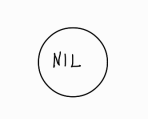
\includegraphics[scale=0.3]{img/ccs/nil.png}
              \caption{Rappresentazione grafica dell'operazione Nil}
          \end{figure}
    \item \textbf{Prefisso}: in cui si ha $\alpha \cdot P$ dove $P \in Proc_{CCS}$
          e $\alpha \in Act$. Questo può essere rappresentato mediante inferenza nel
          seguente modo:
          \begin{equation}
              \frac{}{\alpha \cdot P \xrightarrow{\alpha} P}
          \end{equation}
          \begin{figure}[!ht]
              \centering
              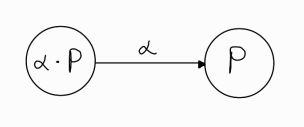
\includegraphics[scale=0.5]{img/ccs/prefisso.png}
              \caption{Rappresentazione grafica dell'operatore prefisso}
          \end{figure}
    \item \textbf{Somma}: siano $p_1, p_2 \in Proc_{CCS}$ posso comporli utilizzando
          l'operatore $+$ nel seguente modo $p_1 + p_2$. In questo caso per definire
          le regole di inferenza necessito $\alpha, \beta \in Act$ e $p_1', p_2' \in Proc_{CCS}$:
          \begin{equation}
              \frac{p_1 + p_2 \xrightarrow{\alpha} p_1'}{p_1 + p_2 \xrightarrow{\alpha} p_1'}
              \ \ \lor \ \
              \frac{p_1 + p2 \xrightarrow{\beta} p_2'}{p_1 + p_2 \xrightarrow{\beta} p_2'}
          \end{equation}
          \begin{figure}[!ht]
              \centering
              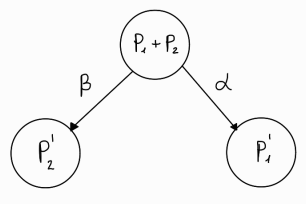
\includegraphics[scale=0.5]{img/ccs/somma.png}
              \caption{Rappresentazione grafica dell'operatore prefisso}
          \end{figure}
          Questo caso può essere generalizzato per più processi. Posso avere
          $\sum_{i \in I} p_i$ avendo multiple somme di processi:
          \begin{equation}
              \frac{p_j \xrightarrow{\alpha} p_j'}{\sum_{i \in I} p_i \xrightarrow{\alpha} p_j'}, \ j \in J
          \end{equation}
          Nel caso di $I = \emptyset$ avrò $\sum_{i \in I} p_i = Nil$. Nell'applicazione
          di questa operazione possono presentarsi situazioni di non determinismo,
          ad esempio avendo $p_1 = \alpha \cdot p_1'$ e $p_2 = \alpha \cdot p_2'$.
    \item \textbf{Composizione parallela}: indicata con il simbolo $p_1 | p_2$ e
          utilizzando le regole di inferenza:
          \begin{equation}
              \frac{p_1 \xrightarrow{\alpha} p_1'}{p_1 | p_2 \xrightarrow{\alpha} p_1' | p_2}
              \ \ \lor \ \
              \frac{p_2 \xrightarrow{\alpha} p_2'}{p_1 | p_2 \xrightarrow{\alpha} p_1 | p_2'}
              \ \ \lor \ \
              \frac{p_1 \xrightarrow{\alpha} p_1' \land p_2 \xrightarrow{\overline{\alpha}} p_2'}{p_1 | p_2 \xrightarrow{\tau} p_1' | p_2'}
          \end{equation}
          in quest'ultimo caso, non potremo più avere altre sincronizzazioni.
          \begin{figure}[!ht]
              \centering
              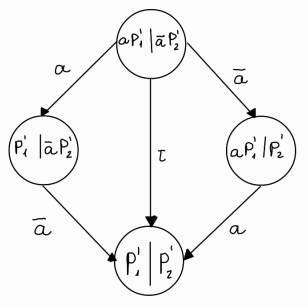
\includegraphics[scale=0.5]{img/ccs/parallela.png}
              \caption{Rappresentazione grafica dell'operatore prefisso}
          \end{figure}
    \item \textbf{Restrizione}: sia $L \subseteq A$. Si ha che:
          \begin{equation}
              p_{\setminus L}
          \end{equation}
          indica che il processo $p$ \textbf{non} può interagire con il suo
          ambiente con azioni in $L \cup \overline{L}$ ma le azioni in
          $L \cup \overline{L}$ sono locali a $p$:
          \begin{equation}
              \frac{p \xrightarrow{\alpha} p'}{ p_{\setminus L} \xrightarrow{\alpha} p'_{\setminus L}}
          \end{equation}
    \item \textbf{Rietichettatura}: ovvero il cambiamento di nome ad una
          componente, ad una certa azione, per poter riusare tale nome. Ho quindi una
          funzione $f$ tale che:
          \begin{equation}
              f: Act \to Act
          \end{equation}
          inoltre, deve sempre essere garantito che:
          \begin{itemize}
              \item $f(\tau) = \tau$
              \item $f(\overline{a}) = \overline{f(a)}$
          \end{itemize}
          Ho quindi $p_{[f]}$ tale che:
          \begin{equation}
              \frac{p \xrightarrow{\alpha} p'}{p_{[f]} \xrightarrow{f(a)} p_{[f]}'}
          \end{equation}
    \item $K = P$ con $K$ uguale al nome di processo e $P \in Proc_{CCS}$:
          \begin{equation}
              \frac{P \xrightarrow{\alpha} P' \land K = P}{K \xrightarrow{\alpha} P'}
          \end{equation}
\end{itemize}
Quindi dato un CCS posso associare un LTS per quanto riguarda la semantica. Si
ha una precedenza degli operatori, da quello con più precedenza a quello con meno precedenza:
\begin{enumerate}
    \item Restrizione
    \item Rietichettatura
    \item Prefisso
    \item Composizione parallela
    \item Somma
\end{enumerate}
\begin{esempio} [\textbf{Priorità degli operatori}]
    Avendo: $$R + a \cdot p | b \cdot Q_{\setminus L}$$ sarebbe: $$R + ((a \cdot p) | b \cdot (Q_{\setminus L}))$$
\end{esempio}
Nel caso di composizione parallela posso eseguire le due operazioni o in una
sequenza o nell'altra. Ho quindi una simulazione sequenziale non deterministica
del comportamento del sistema dato dalla composizione parallela.

Per poter dire che una certa implementazione soddisfa ($\models$) una certa
specifica o se due implementazioni diverse soddisfano la stessa specifica ci
serve una relazione di equivalenza tra processi CCS, ovvero una relazione del
tipo:
\begin{equation}
    R \subseteq Proc_{ccs} \times Proc_{ccs}
\end{equation}
tale che sia \textit{riflessiva}, \textit{simmetrica} e \textit{transitiva}.

Bisognerà inoltre astrarre:
\begin{itemize}
    \item Gli stati e considerare le azioni $Act$.
    \item Dalle sincronizzazioni interne, ovvero dalle $\tau$.
    \item Rispetto al non determinismo.
\end{itemize}
Milner poi asserisce che $R$ deve essere inoltre una \textbf{congruenza} rispetto
agli operatori del CCS.
\begin{definizione}[\textbf{Congruenza}]
    Una relazione di equivalenza $R$ è una \textbf{congruenza} se e solo se:
    \begin{equation}
        \forall p, q \in Proc_{CCS} \land \forall c[\cdot] \ \text{contesto} \ CCS
    \end{equation}
    avendo quindi un \textbf{contesto}, un'espressione CCS con qualcosa di mancante, CCS
    sostituibile con qualcosa, allora:
    \begin{equation}
        \text{se} \ p\ R\ q \ \text{allora si ha} \ c[p] \ R \ c[q]
    \end{equation}
\end{definizione}
Dati due sistemi di transione etichettati $LTS_1 = (Q_1, Act_1, T_1, q_{01})$ e $LTS_1 = (Q_2, Act_2, T_2, q_{02})$,
possiamo affermare che $LTS_1$ è \textbf{isomorfo} a $LTS_2$ se e solo se esistono due funzioni:
\begin{equation}
    \alpha: Q_1 \to Q_2 \ \ \land \ \ \beta: Act_1 \to Act_2
\end{equation}
che sono corrispondenze biunivoche. E se valgono le seguenti assunzioni:
\begin{itemize}
    \item $\alpha(q_{01}) = q_{02}$
    \item $(q_1, a, q_1') \in T_1$ allora $(\alpha(q_1), \beta(a), \alpha(q_1')) \in T_2$
\end{itemize}
\begin{teorema}[\textbf{Equivalenza tra processi CCS}]
    Dati due processi $p_1$ e $p_2$ a cui assegniamo i due LTS $LTS_1$ e $LTS_2$.
    I due processi sono \textbf{equivalenti} se $LTS_1$ e $LTS_2$ sono isomorfi.
\end{teorema}
Oltre all'isomorfismo, due processi sono equivalenti se i due LTS ammettono le
stesse sequenze di operazioni, prendendo l'equivalenza forte tra automi a stati
finiti. Questa è detta \textbf{equivalenza rispetto alle tracce}, ovvero due
programmi sono equivalenti se implementano la stessa sequenza di istruzioni.

Preso $p \in Proc_{CCS}$ posso definire l'insieme delle tracce di $p$ come:
\begin{equation}
    tracce(p) = \{w \in Act^{\ast}\ |\ \exists p' \in Proc_{CCS} \ p \xrightarrow{w} p'\}
\end{equation}
Suppongo, per ora, di non considerare le sincronizzazioni (quindi senza $\tau$).
\begin{itemize}
    \item Se $w = \varepsilon$ allora $p =  p'$
    \item Se $w = x_1 \cdot x_2 \cdot \dots \cdot x_n$ con $x_i \in Act$
          $\exists p_1', p_2', \dots, p_n' \in Proc_{CCS}$ tale che:
          $$p \xrightarrow{x_1} p_1' \xrightarrow{x_2} \dots \xrightarrow{x_n} p_n' = p'$$
\end{itemize}
\begin{teorema}[\textbf{Equivalenza rispetto alle tracce}]
    Preso $p' \in Proc_{CCS}$ è \textbf{equivalente rispetto alle tracce} a $p''$,
    indicato come $p' \stackrel{T}{\sim}  p''$ se e solo se:
    \begin{equation}
        tracce(p') = tracce(p'')
    \end{equation}
\end{teorema}
Lo studio delle tracce non è più sufficiente nel caso di sistemi concorrenti.
Si necessità quindi di una nozione più restrittiva.
\subsection{Bisimulazione forte}
Dato che le tracce non sono sufficienti nel caso di processi concorrenti, si
definisce il concetto di \textbf{bisimulazione}.
\begin{definizione}[\textbf{Relazione di Bisimulazione Forte}]
    Data una relazione binaria $R \subseteq Proc_{CCS} \times Proc_{CCS}$ è una
    relazione di \textbf{bisimulazione} (\textbf{forte}) se e solo se
    $\forall p, q \in Proc_{CCS}: \ p R q$ vale che:
    \begin{itemize}
        \item $\forall \alpha \in Act = A \cup \overline{A} \cup \{\tau\}$ se ho
              $p \xrightarrow{\alpha} p'$ allora deve esistere un processo
              \begin{equation}
                  \exists q' \ \text{tale che} \ q \xrightarrow{\alpha} q' \ \text{e si ha} \ p'Rq'
              \end{equation}
        \item E viceversa, ovvero $\forall \alpha \in Act = A \cup \overline{A} \cup \{\tau\}$
              se ho $q \xrightarrow{\alpha} q'$ allora deve esistere un processo
              \begin{equation}
                  \exists p' \ \text{tale che} \ p \xrightarrow{\alpha} p' \ \text{e si ha} \ p'Rq'
              \end{equation}
    \end{itemize}
    Due processi $p$ e $q$ sono fortemente bisimili, indicato con la notazione
    $p \stackrel{Bis}{\sim} q$ se e solo se $\exists R \subseteq Proc_{CCS} \times Proc_{CCS}$,
    relazione di bisimulazione forte tale che:
    \begin{equation}
        p R q \ \ \land \ \
        \stackrel{Bis}{\sim} = \bigcup \{R \subseteq Proc_{CCS} \times Proc_{CCS} \ | \ R \ \text{è una relazione di bisimulazione forte}\}
    \end{equation}
\end{definizione}
\begin{teorema}
    Se prendo $\stackrel{Bis}{\sim}  \subseteq Proc_{CCS} \times Proc_{CCS}$ si
    dimostra che è una relazione di equivalenza, ovvero è riflessiva, simmetrica
    e transitiva. Quindi:
    \begin{equation}
        p \stackrel{Bis}{\sim} q \Longleftrightarrow \forall \alpha \in Act \ \text{se} \ p \xrightarrow{\alpha} p'
        \ \text{allora} \
        \exists q' \ \text{tale che} \ q \xrightarrow{\alpha} q' \ \land \ p' \stackrel{Bis}{\sim} q'
    \end{equation}
    e se:
    \begin{equation}
        q \xrightarrow{\alpha} q' \ \text{allora} \
        \exists p' \ \text{tale che} \ p \xrightarrow{\alpha} p' \ \land \ p' \stackrel{Bis}{\sim} q'
    \end{equation}
\end{teorema}
\begin{teorema}
    Se due processi sono fortemente bisimili allora sono sicuramente equivalenti
    rispetto alle tracce. Non vale il viceversa.
\end{teorema}
\begin{osservazione}
    Per vedere che due processi sono bisimili devo quindi, per ogni esecuzione,
    ottenere due processi ancora bisimili (potendo quindi fare le azioni
    corrispondenti da entrambe le parti).
\end{osservazione}
\begin{esempio}
    Consideriamo i processi $p_1 = a \cdot b \cdot Nil + a \cdot c \cdot Nil$ e
    $p_2 = a \cdot (b \cdot Nil + c \cdot Nil)$
    \begin{figure}[!ht]
        \centering
        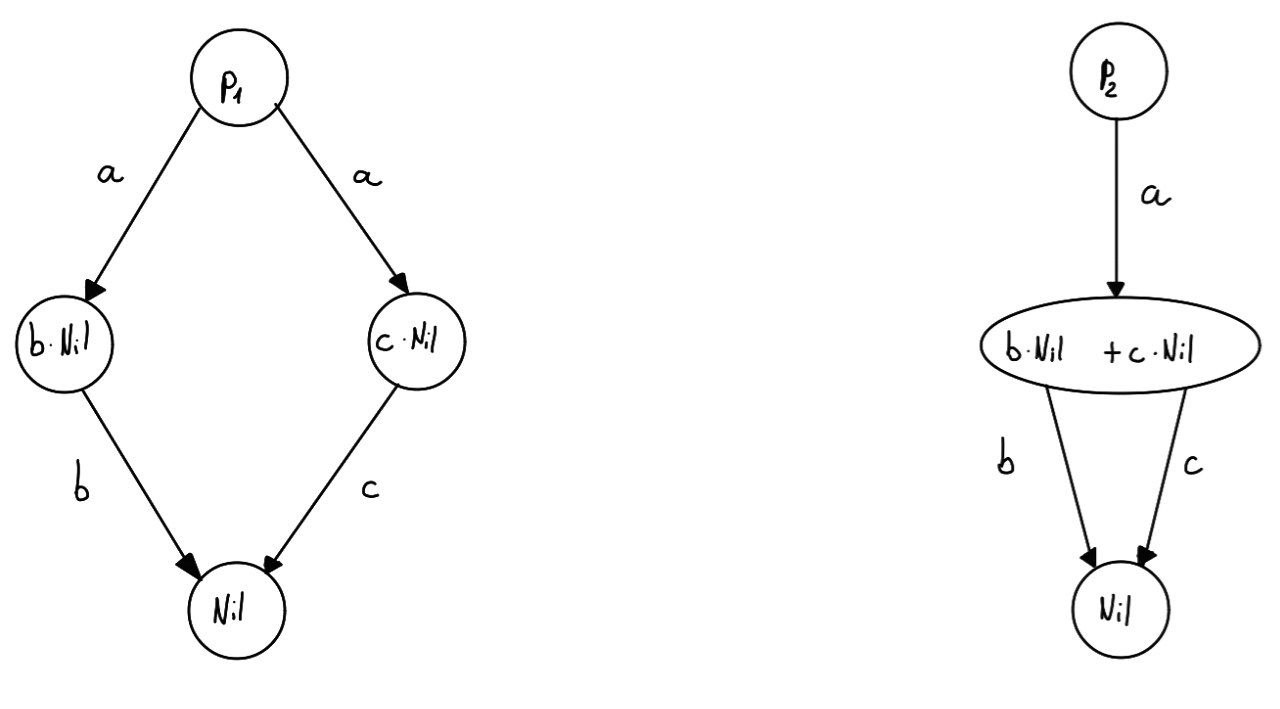
\includegraphics[scale=0.25]{img/ccs/Esempio1.png}
        \caption{LTS dei processi $p_1$ e $p_2$}
    \end{figure}
    Osserviamo subito che i due processi sono equivalenti rispetto alle tracce,
    difatti:
    \begin{itemize}
        \item $Tracce(p_1) = \{\varepsilon, a, a \cdot b, a \cdot c\}$
        \item $Tracce(p_2) = \{\varepsilon, a, a \cdot b, a \cdot c\}$
    \end{itemize}
    Vediamo se i due processi sono anche bisimili.
    \begin{itemize}
        \item Da $p_1$ possiamo eseguire l'azione $a$ e possiamo fare lo stesso
              anche da $p_2$. Dobbiamo però chiederci se gli stati di arrivo sono anche
              essi in relazione di bisimulazione.
        \item Gli stati interessati sono $b \cdot Nil$ e $b \cdot Nil + c \cdot Nil$:
              dal primo possiamo eseguire $b$, che è fattibile anche dal secondo, ma
              dal secondo possiamo eseguire $c$, che non è eseguibile dal primo (la
              bisimulazione richiede che entrambi gli stati siano simili tra loro),
              dunque i due processi non sono bisimili.
    \end{itemize}
    Formalmente:
    \begin{itemize}
        \item $p_1 \xrightarrow{a} b \cdot Nil$
        \item $p_2 \xrightarrow{a} b \cdot Nil + c \cdot Nil$
    \end{itemize}
    $b \cdot Nil \stackrel{Bis}{\not\sim} b \cdot Nil + c \cdot Nil$ inoltre,
    possiamo osservare che: $b \cdot Nil \stackrel{T}{\not\sim} b \cdot Nil + c \cdot Nil$
\end{esempio}
\begin{esempio}
    Consideriamo due processi che simulano dei buffer che possono contenere due
    elementi:
    \begin{itemize}
        \item $B_0^1 | B_0^1$ dove $B_0^1 = in \cdot B_1^1$ e $B_1^1 = \overline{out} \cdot B_0^1$
        \item $B_0^2 = in \cdot B_1^2$, $B_1^2= \overline{out} \cdot B_0^2 + in \cdot B_2^2$ e $B_2^2 = \overline{out} \cdot B_1^2$
    \end{itemize}
    \begin{figure}[!ht]
        \centering
        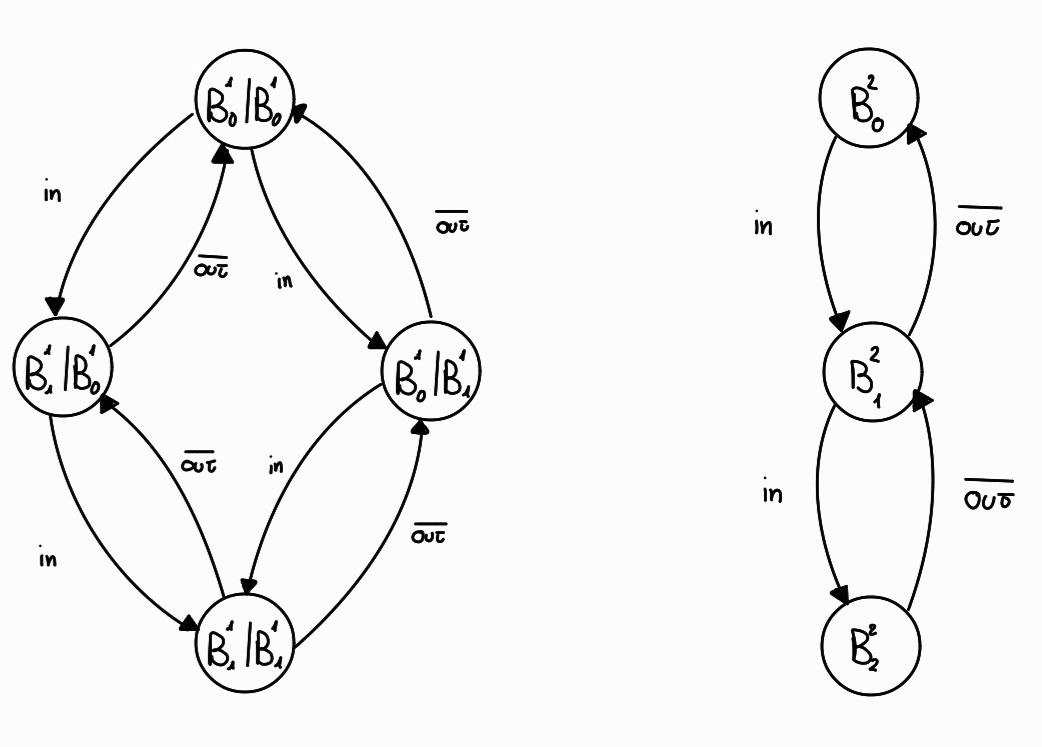
\includegraphics[scale=0.25]{img/ccs/Esempio 2.png}
        \caption{LTS dei processi $B_0^1 | B_0^1$ e $B_0^2$}
    \end{figure}
    In questo esempio, possiamo osservare che: $$(B_0^1 | B_0^1) \stackrel{Bis}{\sim} B_0^2$$
    $B_0^2$ può essere messo in relazione con $B_0^1| B_0^1$ in quanto se vado
    in uno tra $B_1^1 | B_0^1$ e $B_0^1 | B_1^1$ posso sempre fare $in$ e $\overline{out}$.
    Inoltre, Posso fare un discorso analogo per $B_2^2$ e $B_1^1 | B_1^1$.
    Essendo questi ultimi quindi bisimili lo sono anche il nodo centrale coi
    due possibili nodi nel caso della composizione e di conseguenza lo sono
    anche $B_0^2$ e $B_0^1 | B_0^1$.
\end{esempio}
Cerco quindi di astrarre dalle interazioni interne ($\tau$), introducendo
l'equivalenza debole, volendo astrarre rispetto alle azioni $\tau$ , introducendo
il concetto di bisimulazione debole.

Vediamo quindi le proprietà della bisimulazione forte:
\begin{itemize}
    \item La bisimulazione forte è una congruenza rispetto agli operatori del CCS.
          Quindi se ho $p \stackrel{Bis}{\sim} q$ con $p, q \in Proc_{CCS}$ vale:
          $$\alpha \cdot p \stackrel{Bis}{\sim}  \alpha \cdot q \ \forall \ \alpha \in Act$$
    \item Vale la proprietà commutativa rispetto alla composizione $+$:
          $$p + r \stackrel{Bis}{\sim} q + r \ \land \ r + p \stackrel{Bis}{\sim} r + q, \ \ \forall r \in Proc_{CCS}$$
    \item Vale la proprietà commutativa rispetto alla composizione $|$:
          $$p | r \stackrel{Bis}{\sim} q | r \ \land \ r | p \stackrel{Bis}{\sim} r | q, \ \ \forall r \in Proc_{CCS}$$
    \item Per ogni funzione di rietichettatura $f : Act \to Act$ vale:
          $$p_{[f]} \stackrel{Bis}{\sim} q_{[f]}$$
    \item $p_{\backslash L} \stackrel{Bis}{\sim} q_{\backslash L}$
\end{itemize}
A queste proprietà possiamo aggiungere delle \textit{leggi} legate al fatto che
gli operatori hanno delle proprietà. Dati $p, q, r \in Proc_{CCS}$ valgono le seguenti proprietà:
\begin{itemize}
    \item \textbf{Commutatività}: $$p + q \stackrel{Bis}{\sim} q + p \ \land \ p | q \stackrel{Bis}{\sim} q | p$$
    \item \textbf{Distributività}: $$(p + q) + r \stackrel{Bis}{\sim} p + (q + r) \ \land \ (p | q) | r \stackrel{Bis}{\sim} p | (q | r)$$
    \item \textbf{Leggi di assorbimento}: $$p + Nil \stackrel{Bis}{\sim} p \ \land \ p | Nil \stackrel{Bis}{\sim} p$$
\end{itemize}
\subsection{Bisimulazione debole}
La bisimulazione forte rischia di essere troppo restrittiva. Si passa quindi alla
definizione di \textbf{equivalenza debole rispetto alle tracce} $\stackrel{T}{\approx}$
e \textbf{bisimulazione debole} $\stackrel{Bis}{\approx}$.
La definizione di queste nuove relazioni obbliga a modificare la definizione
della funzione di transizione. La relazione di transizione debole è definita come:
\begin{equation}
    \Rightarrow \subseteq Proc_{CCS} \times Act \times Proc_{CCS}
\end{equation}
Possiamo rappresentare tale funzione come $p \stackrel{\alpha}{\Rightarrow} p'$ dove
$\alpha \in Act$ se e solo se:
\begin{itemize}
    \item Se $\alpha = \tau$ allora posso eseguire una sequenza qualsiasi, anche
          nulla, di $\tau$: $$p \xrightarrow{\tau}^{\ast} p'\begin{cases}
                  p = p'                                                                  & \text{se non ci sono } \tau \text{ da eseguire} \\
                  p \xrightarrow{\tau} p_1 \xrightarrow{\tau} \dots \xrightarrow{\tau} p' & \text{altrimenti}
              \end{cases}$$
    \item Se $\alpha \in A \cup \overline{A}$ allora vale:
          $p \xrightarrow{\tau}^{\ast} \xrightarrow{\alpha} \xrightarrow{\tau}^{\ast}$
\end{itemize}
Come fatto per la relazione forte, definiamo la relazione di transizione per
sequenze di azioni $w \in Act^{\ast}$ come $p \stackrel{w}{\Rightarrow} p'$ se e solo se:
\begin{itemize}
    \item Se $w = \varepsilon$ oppure $w = \tau^{\ast}$ allora ho: $$p \xrightarrow{\tau}^{\ast} p'$$
    \item Se $w = a_1\dots a_n$ con $a_i \in A \cup \overline{A}$ allora:
          $$p \stackrel{a_1}{\Rightarrow} p_1 \stackrel{a_2}{\Rightarrow} \dots \stackrel{a_n}{\Rightarrow} p'$$
          dove ogni $a_i$ può essere preceduto/seguito da una qualsiasi sequenza di $\tau$.
\end{itemize}
\begin{definizione}[\textbf{Equivalenza debole rispetto alle tracce}]
    Definiamo l'\textbf{equivalenza debole rispetto alle tracce}, la quale è
    rappresentata come $p \stackrel{T}{\approx} q$ se e solo se:
    \begin{equation}
        tracce_{\Rightarrow} (p) = tracce_{\Rightarrow}(q) \ \text{ovvero} \
        \forall w \in (A \cup \overline{A}) \ \text{ho che} \ p \stackrel{w}{\Rightarrow}
        \iff q \stackrel{w}{\Rightarrow}
    \end{equation}
    quindi se i due processi possono eseguire la stessa sequenza di azioni.
\end{definizione}
Posso definire le tracce come:
\begin{equation}
    tracce_{\Rightarrow}(p) = \{w \in (A \cup \overline{A})^{\ast} | p \stackrel{w}{\Rightarrow}\}
\end{equation}
\begin{definizione}
    Data una relazione $R$ definita come $R \subseteq Proc_{CCS} \times Proc_{CCS}$.
    Dico che $R$ è una relazione di \textbf{bisimulazione debole} se e solo se:
    \begin{equation}
        \forall p, q \in Proc_{CCS} \ \text{tale che } p R q \ \text{vale che } \forall a \in Act
    \end{equation}
    \begin{itemize}
        \item Se $p \xrightarrow{a} p'$ allora $\exists q'$ tale che
              $q \stackrel{a}{\Rightarrow} q'$ e $p'Rq'$
        \item E deve valere anche il viceversa: $q \xrightarrow{a} q'$ allora
              $\exists p'$ tale che $p \stackrel{a}{\Rightarrow} p'$ e $p'Rq'$
    \end{itemize}
\end{definizione}
Due processi $p$ e $q$ sono in relazione di bisimulazione debole $p \stackrel{Bis}{\approx} q$
se e solo se esiste una relazione di bisimulazione $R$ tale che $p R q$ si ha che vale:
\begin{equation}
    \stackrel{Bis}{\approx} = \bigcup \{R | R \ \text{è di bisimulazione debole}\}
\end{equation}
\begin{esempio}
    Consideriamo i processi $r = a \cdot (b \cdot Nil + \tau \cdot c \cdot Nil)$
    e $k = a \cdot (b \cdot Nil + \tau \cdot c \cdot Nil) + a \cdot c \cdot Nil$.
    \begin{figure}[!ht]
        \centering
        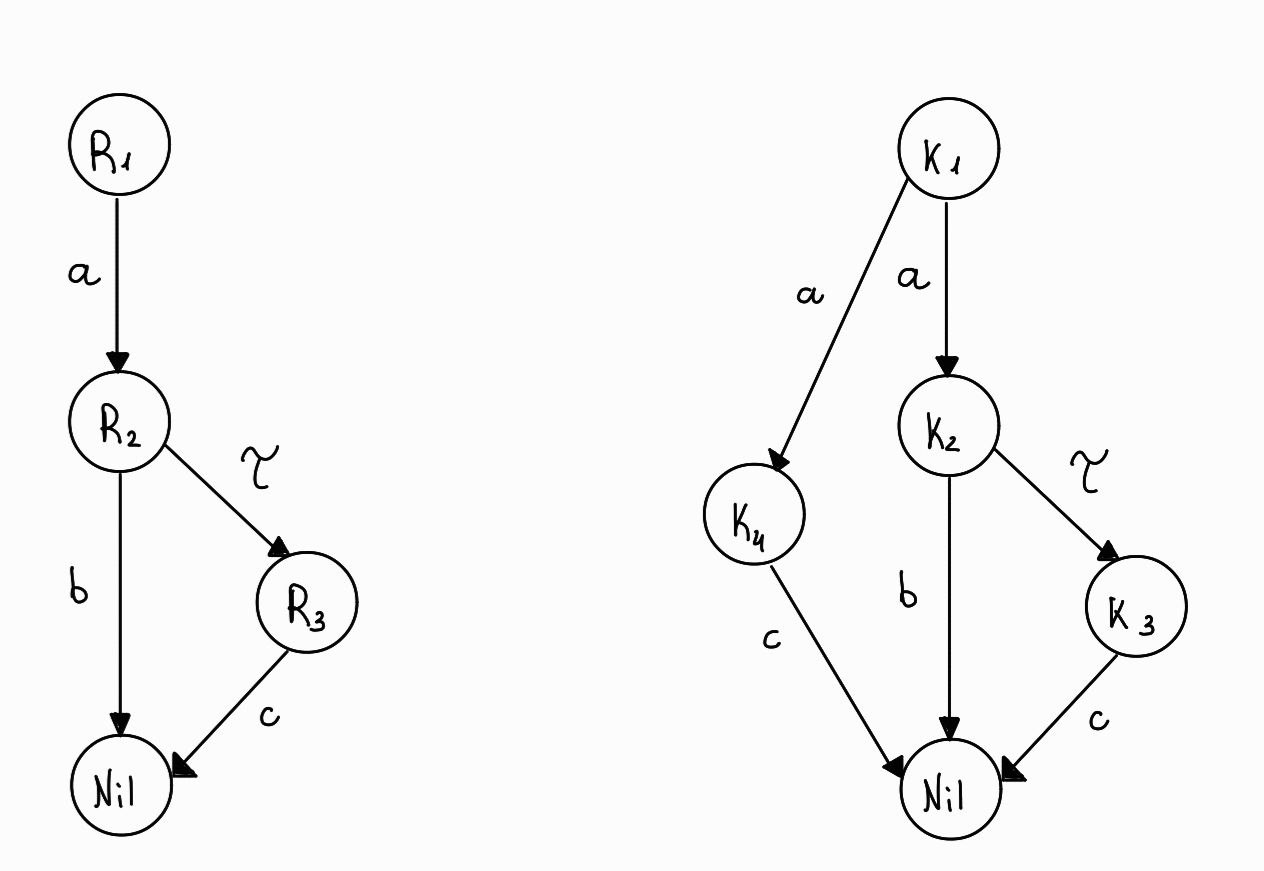
\includegraphics[scale=0.25]{img/ccs/Esempio3.png}
        \caption{LTS di $r$ e $k$}
    \end{figure}
    $$r \stackrel{Bis}{\approx} k$$
\end{esempio}
\subsubsection{Gioco verifica bisimulazione debole}
Per confrontare due processi $p$ e $q$ si può utilizzare un gioco $G(p, q)$ con
2 giocatori:
\begin{itemize}
    \item \textbf{Attaccante}: il quale cerca di dimostrare che $p \stackrel{Bis}{\not\approx} q$
    \item \textbf{Difensore}: il quale cerca di dimostrare che $p \stackrel{Bis}{\approx} q$
\end{itemize}
Un gioco è composto da più partite, dove ogni partita è una sequenza finita o
infinita di configurazioni: $$(p_0, q_0), (p_1, q_1), \dots, (p_i, q_i), \dots$$
In ogni mano si passa dalla configurazione corrente $(p_i, q_i)$ alla successiva
$(p_{i + 1}, q_{i + 1})$ con le seguenti regole:
\begin{itemize}
    \item L'Attaccante sceglie uno dei due processi della configurazione corrente
          $(p_i, q_i)$ e fa una $\xrightarrow{\alpha}$ mossa $(\alpha \in Act)$
    \item Il Difensore deve rispondere con una $\stackrel{\alpha}{\Rightarrow}$
          mossa nell'altro processo.
\end{itemize}
La coppia di processi $(p_{i+1}, q_{i+1})$ così ottenuta diventa la nuova
configurazione corrente. La partita continua con un'altra mano.

La partita può terminare in uno dei due seguenti modi:
\begin{itemize}
    \item Se un giocatore non può muovere, l'altro vince.
    \item Se la partita è infinita, vince il difensore.
\end{itemize}
Diverse partite possono concludersi con vincitori diversi, ma per ogni gioco, un
solo giocatore può vincere ogni partita.

Una \textbf{strategia} per un giocatore è un insieme di regole che indicano di
volta in volta che mossa fare. Tali regole dipendono solo dalla configurazione
corrente. Un giocatore ha una \textbf{strategia vincente} per un gioco $G(p, q)$
se seguendo quella strategia è in grado di vincere tutte le partite del gioco.
\begin{teorema}
    Per ogni gioco $G(p, q)$, solo uno dei due giocatori ha una strategia vincente.
    \begin{itemize}
        \item L'Attaccante ha una strategia vincente per $G(p, q)$ se e solo se
              $p \stackrel{Bis}{\not\approx} q$.
        \item Il Difensore ha una strategia vincente per $G(p, q)$ se e solo se
              $p \stackrel{Bis}{\approx} q$.
    \end{itemize}
\end{teorema}
\begin{nota}
    Il gioco della bisimulazione può essere usato sia per dimostrare che due
    processi sono bisimili, che per dimostrare che non lo sono.
\end{nota}
Per dimostrare che i processi sono bisimili, bisogna mostrare che il Difensore
ha una strategia vincente, cioè che, per ogni mossa dell'Attaccante, il Difensore
ha almeno una mossa che lo porterà a vincere.

Per dimostrare che i processi \textbf{non} sono bisimili, bisogna mostrare che
l'Attaccante ha una strategia vincente, cioè che, in ogni configurazione,
l'Attaccante è in grado di scegliere su quale processo operare e con quale azione,
in modo che per ogni successiva mossa del Difensore, l'Attaccante ha almeno una
mossa che lo porterà a vincere.
\section{Proprietà}
Siano $p, q \in Proc_{CCS}$:
\begin{itemize}
    \item Se $LTS(p)$ è isomorfo a $LTS(q)$ allora $p \simeq q$.
    \item Deve astrarre dagli stati.
    \item Se $p \simeq q$ allora le tracce di $p$ e $q$ sono equivalenti
          $Tracce(p) = Tracce(q)$.
    \item Se $p \simeq q$ allora $p$ e $q$ devono avere la stessa possibilità di
          generare deadlock nell'interazione con l'ambiente.
    \item $\simeq$ deve essere una congruenza rispetto agli operatori CCS: deve
          essere possibile sostituire un sotto-processo con un suo equivalente senza
          modificare il comportamento complessivo del sistema.
\end{itemize}
Siano $p, q \in Proc_{CCS}$ l'equivalenza rispetto alle tracce forte gode delle
seguenti proprietà:
\begin{itemize}
    \item Se $LTS(p)$ è isomorfo a $LTS(q)$ allora $p \stackrel{T}{\sim} q$.
    \item Astrae dagli stati.
    \item Se $p \stackrel{T}{\sim} q$ se e solo se le tracce di $p$ e $q$ sono
          equivalenti $Tracce(p) = Tracce(q)$.
    \item $\stackrel{T}{\sim}$ è una congruenza rispetto agli operatori CCS.
    \item Non garantisce di preservare il deadlock o l'assenza di deadlock,
          nell'interazione con l'ambiente.
\end{itemize}
Siano $p, q \in Proc_{CCS}$ la bisimulazione forte gode delle seguenti proprietà:
\begin{itemize}
    \item Se $LTS(p)$ è isomorfo a $LTS(q)$ allora $p \stackrel{Bis}{\sim} q$.
    \item Astrae dagli stati.
    \item Se $p \stackrel{Bis}{\sim} q$ se le tracce di $p$ e $q$ sono equivalenti
          $Tracce(p) = Tracce(q)$.
    \item $\stackrel{Bis}{\sim}$ è una congruenza rispetto agli operatori CCS.
    \item Preservare il deadlock o l'assenza di deadlock, nell'interazione con
          l'ambiente.
\end{itemize}
L'equivalenza rispetto alle Tracce forte è più restrittiva dell'equivalenza
rispetto alle Tracce debole. Siano $p, q \in Proc_{CCS}$ l'equivalenza rispetto
alle tracce debole gode delle seguenti proprietà:
\begin{itemize}
    \item Se $LTS(p)$ è isomorfo a $LTS(q)$ allora $p \stackrel{T}{\approx} q$.
    \item Astrae dagli stati.
    \item Se $p \stackrel{T}{\approx} q$ se e solo se le tracce di $p$ e $q$ sono
          equivalenti $Tracce(p) = Tracce(q)$.
    \item $\stackrel{T}{\approx}$ è una congruenza rispetto agli operatori CCS.
    \item Non garantisce di preservare il deadlock o l'assenza di deadlock,
          nell'interazione con l'ambiente.
\end{itemize}
La bisimulazione forte è più restrittiva della bisimulazione debole:
\begin{equation}
    p \stackrel{Bis}{\sim} q \Rightarrow p \stackrel{Bis}{\approx} q
    \ (\stackrel{Bis}{\sim} \subseteq \stackrel{Bis}{\approx})
\end{equation}
La bisimulazione forte (debole) è più restrittiva dell'equivalenza rispetto alle
Tracce forte (debole)
\begin{equation}
    p \stackrel{Bis}{\sim} q \Rightarrow p \stackrel{T}{\sim} q \ e
    \ p \stackrel{Bis}{\approx} q \Rightarrow p \stackrel{T}{\approx} q
\end{equation}
\begin{equation}
    (\stackrel{Bis}{\sim} \subseteq \stackrel{T}{\sim}) \ e \
    (\stackrel{Bis}{\approx} \subseteq \stackrel{T}{\approx})
\end{equation}
\begin{definizione}[\textbf{Processo deterministico}]
    $p \in Proc_{CCS}$ è un processo deterministico se e solo se vale che:
    \begin{equation}
        \forall x \in Act = A \cup \overline{A} \cup \{\tau\}, \ \text{se} \ p
        \xrightarrow{\ast} p' \ \text{e} \ p \xrightarrow{\ast} p'' \ \text{allora} \ p' = p''
    \end{equation}
\end{definizione}
Siano $p, q \in Proc_{CCS}$ se $p$ e $q$ sono deterministici e
$p \stackrel{T}{\sim} q$ ($p \stackrel{T}{\approx} q$) allora
$p \stackrel{Bis}{\sim} q$ ($p \stackrel{Bis}{\approx} q$).

Siano $p, q \in Proc_{CCS}$ la bisimulazione debole gode delle seguenti proprietà:
\begin{itemize}
    \item È un'equivalenza, la più grande relazione di Bisimulazione debole.
    \item Astrae da azioni non osservabili ($\tau$) e dai cicli inosservabili ($\tau \ loop$).
    \item Preservare il deadlock o l'assenza di deadlock, nell'interazione con l'ambiente.
\end{itemize}
\begin{teorema}
    Se $p, q \in Proc_{CCS}$ tale che $p \stackrel{Bis}{\approx} q$, allora:
    \begin{itemize}
        \item $\alpha \cdot p \stackrel{Bis}{\approx} \alpha \cdot q \ \ \ \forall \alpha \in A_{CCS} = A \cup \overline{A} \cup \tau$
        \item $p | r \stackrel{Bis}{\approx} q | r \ \land \ r | p \stackrel{Bis}{\approx} r | q$ $\forall r \in Proc_{CCS}$
        \item $p_{[f]} \stackrel{Bis}{\approx} q_{[f]}$ $\forall f$ funzione di
              etichettatura.
        \item $p_{\backslash L} \stackrel{Bis}{\approx} q_{\backslash L}$ $\forall L \subseteq A$
    \end{itemize}
    La Bisimulazione debole è una congruenza rispetto agli operatori del CCS
    diversi da $+$ e ricorsione.

    Posso quindi affermare che la Bisimulazione debole non è una congruenza per
    il CCS.
\end{teorema}
\section{Congruenza}
Si definisce quindi, tramite assiomi, la più grande relazione di congruenza
$\stackrel{C}{\approx}$ (per il CCS puro e senza ricorsione, con agenti finiti)
che è contenuta nella relazione di Bisimulazione $\stackrel{Bis}{\approx}$.
\begin{equation}
    \stackrel{C}{\approx} \subseteq \stackrel{Bis}{\approx} \subseteq Proc_{CCS} \times Proc_{CCS}
\end{equation}
insieme finito di Assiomi $Ax$:
\begin{itemize}
    \item Ax \textit{corretto} ($Ax \vdash p = q \Rightarrow p \stackrel{C}{\approx} q$)
    \item Ax \textit{completo} ($p \stackrel{C}{\approx} q \Rightarrow Ax \vdash p = q$)
\end{itemize}
\begin{enumerate}
    \item $p + (q + r) \stackrel{C}{\approx} (p + q) + r$ e $p | (q | r) \stackrel{C}{\approx} (p | q) | r$
    \item $p + q \stackrel{C}{\approx} q + p$ e $p | q \stackrel{C}{\approx} q | p$
    \item $p + p \stackrel{C}{\approx} p$ (ma $p | p \stackrel{C}{\not\approx} p$)
    \item $p + Nil \stackrel{C}{\approx} p$ e $p | Nil \stackrel{C}{\approx} p$
    \item $p + \tau \cdot p \stackrel{C}{\approx} \tau \cdot p$
    \item $\mu \cdot \tau p \stackrel{C}{\approx} \mu \cdot p$
    \item $\mu \cdot (p + \tau \cdot q) \stackrel{C}{\approx} \mu \cdot (p + \tau \cdot q) + \mu \cdot q$
    \item Se $p$ e $q$ sono delle somme: $p = \sum_{i} \alpha_i \cdot p_i$ e
          $q = \sum_{j} \beta_j \cdot q_j$,  $\alpha, \beta \in Act$:
          $$p | q \stackrel{C}{\approx} \sum_{i} \alpha_i (p_{i} | q) + \sum_{j} \beta_{j} \cdot (p|q_{j}) + \sum_{\alpha_i = \overline{\beta}_{j}} \tau \cdot (p_{i} | q_{j})$$
          (Teorema di espansione di R. Milner) Questo assioma mi permette di rappresentare
          la composizione parallela come la somma di tutte le possibili alternative
          che si hanno con l'operazione di composizione parallela.
    \item $p[f] \stackrel{C}{\approx} \sum_{i} f(\alpha_i) \cdot (p_{i} [f])$ $\forall f$
          funzione di etichettatura.
    \item $p_{\backslash L} \stackrel{C}{\approx} \sum_{\alpha_i,\overline{\alpha}_i \not\in L} \alpha_i \cdot (pi_{\backslash L})$ $\forall L \subseteq A$
\end{enumerate}
\chapter{Reti di Petri}
Abbiamo introdotto un'algebra di processi come CCS dove processi sequenziali
interagiscono tra loro tramite hand-shaking. Un altro modello usato, con varie
implementazioni, sono gli automi a stati finiti. Si passa ora alle reti di Petri.

La critica di Petri è che in un sistema distribuito non sia individuabile uno
stato globale, che in un sistema distribuito le trasformazioni di stato siano
localizzate e non globali, che non esista un sistema di riferimento temporale
unico. Quindi la simulazione sequenziale non deterministica (semantica a
“interleaving”) dei sistemi distribuiti è una forzatura e non rappresenta le
reali caratteristiche del comportamento del sistema, ovvero la località, la
distribuzione degli eventi e la relazione di dipendenza causale e non causale
tra gli eventi.

Nel modello proposto da Petri, le azioni vengono rappresentate come nodi
dell'automa e non più come etichette della transizione. Oltre a ciò, le azioni e
le coazioni che abbiamo definito in CCS per sincronizzare due processi diventano
una singola azione di sincronizzazione.

Petri sviluppò una teoria matematica fondata sui principi della fisica moderna,
che sia una teoria dei sistemi in grado di descrivere il flusso di informazione
e permetta di analizzare sistemi con organizzazione complessa.

Lo \textbf{stato} è definito da una collezione di stati locali.
\section{Reti elementari}
\begin{definizione}[\textbf{Rete}]
    Una \textbf{rete} è definite come:
    \begin{equation}
        N = (B, E, F)
    \end{equation}
    dove:
    \begin{itemize}
        \item $B$ è un insieme finito di condizioni, anche detti stati locali,
              proposizioni vere o false. Rappresentato da: $$\bigcirc$$
        \item $E$ è un insieme finito di eventi, \textbf{trasformazioni locali}
              di stato. Rappresentato da: $$\Box$$
        \item $F \subseteq (B \times E) \cup (E \times B)$ è una
              \textbf{relazione di flusso} Rappresentato da: $$\to$$
              Inoltre, la relazione di flusso è tale per cui non esistano elementi
              isolati, in quanto non avrebbero senso, in un tale sistema, eventi isolati
              o condizioni isolate. Si ha, formalmente, che:
              \begin{equation}
                  dom(F) \cup ran(F) = B \cup E
              \end{equation}
              ovvero non ho condizioni/eventi isolati, in quanto non avrebbero
              senso, avrei una condizione costante e un evento che non accade
              mai; quindi, dominio e codominio di $F$ coprono l'insieme di
              condizioni ed eventi.
    \end{itemize}
\end{definizione}
Sia $x \in X$ dove l'insieme $X$ è definito come $X = B \cup E$, allora possiamo
definire:
\begin{itemize}
    \item $^{\bullet} x =\{y \in X: \ (y, x) \in F\}$ sono i \textbf{pre-elementi}
          di $x$. Posso anche definirli come precondizioni o pre-eventi.
    \item $x^{\bullet} =\{y \in X: \ (x, y) \in F\}$ sono i \textbf{post-elementi}
          di $x$. Posso anche definirli come post-condizioni o post eventi.
\end{itemize}
Sia $A \subseteq B \cup E$ allora posso definire:
\begin{itemize}
    \item $^{\bullet} A = \bigcup_{x \in A} \ ^{\bullet} x$
    \item $A^{\bullet} = \bigcup_{x \in A} x^{\bullet}$
\end{itemize}
Nelle reti c'è sempre una relazione di dualità tra due elementi, per esempio tra
condizioni ed eventi, tra pre-eventi e post-eventi, tra precondizioni e post
condizioni. Inoltre, si ha la caratteristica della località, quindi si hanno stati
locali e trasformazioni di stato locali.

La rete $N = (B, E, F)$ descrive la struttura statica del sistema, il
comportamento è definito attraverso le nozioni di caso e di regola di scatto o
regola di transizione.

Un \textbf{caso} o \textbf{configurazione} è un insieme di condizioni $c \subseteq B$
che rappresentano l'insieme di condizioni vere in una certa configurazione del
sistema, un insieme di stati locali che collettivamente individuano lo
\textit{stato globale} del sistema.
\begin{itemize}
    \item Condizione vera: $$\bigodot$$
    \item Condizione falsa: $$\bigcirc$$
\end{itemize}
\begin{definizione} [\textbf{Regola dello scatto}]
    Sia $N = (B, E, F)$ una rete elementare e $c \subseteq B$. L'evento $e \in E$
    è \textbf{abilitato}, ovvero può occorrere, in $c$, denotato $c[e >$, se e
    solo se:
    \begin{equation}
        ^{\bullet} e \subseteq c \ \land \ e^{\bullet} \cap c = \emptyset
    \end{equation}
    Se $c[e >$, allora quando $e$ occorrere in $c$ genera un nuovo caso $c'$,
    denotato $c[e > c'$:
    \begin{equation}
        c' = (c - ^{\bullet} e) \cup e^{\bullet}
    \end{equation}
\end{definizione}
In altre parole, un evento $e$ è abilitato se le sue precondizioni sono vere,
le post-condizioni false. Lo scatto di $e$ rende le precondizioni false e le
post-condizioni vere, le altre condizioni rimangono inalterate.

Le reti si basano sul \textbf{principio di estensionalità}, ovvero sul fatto che
il cambiamento di stato è locale:
\begin{center}
    \textit{Un evento è completamente caratterizzato dai cambiamenti che produce
        negli stati locali, tali cambiamenti sono indipendenti dalla particolare
        configurazione in cui l'evento occorre.}
\end{center}
\begin{definizione}[]
    Sia $N = (B, E, F)$ una \textbf{rete elementare}, si ha che:
    \begin{itemize}
        \item $N$ è \textbf{semplice} se e solo se:
              \begin{equation}
                  \forall x, y \in B \cup E, \ ^{\bullet} x = \ ^{\bullet} y \ \land \ x^{\bullet} = y^{\bullet} \Rightarrow x = y
              \end{equation}
        \item $N$ è \textbf{pura} se e solo se:
              \begin{equation}
                  \forall e \in E: \ ^{\bullet}e \cap e^{\bullet} = \emptyset
              \end{equation}
    \end{itemize}
\end{definizione}
\begin{definizione}
    Sia $N = (B, E, F)$ una rete elementare, $U \subseteq E$ e $c, c_1, c_2 \subseteq B$.
    \begin{itemize}
        \item $U$ è un \textbf{insieme di eventi indipendenti} se e solo se:
              \begin{equation}
                  \forall e_1, e_2 \in U: \ e_1 \neq e_2 \Rightarrow (^{\bullet}e_1 \cup e_1^{\bullet}) \cap (^{\bullet}e_2 \cup e_2^{\bullet}) = \emptyset
              \end{equation}
        \item $U$ è un \textbf{passo abilitato} (insieme di eventi concorrenti)
              in $c$ anche scritto come $c[U >$ se e solo se:
              \begin{equation}
                  U \ \text{insieme di eventi indipendenti} \ \land \ \forall e \in U: \ c[e >
              \end{equation}
        \item $U$ è un \textbf{passo} da $c_1$ a $c_2$, anche scritto come
              $c_1[U > c_2$ se e solo se:
              \begin{equation}
                  c_1 [ U > \ \land \ c_2 = (c_1 - \ ^{\bullet} U) \cup U^{\bullet}
              \end{equation}
    \end{itemize}
\end{definizione}
Un \textbf{sistema elementare} $\Sigma = (B, E, F; c_{in})$ è definito da una rete
$N = (B, E, F)$ e da $c_{in} \subseteq B$ un caso iniziale.

L'insieme dei \textbf{casi raggiungibili} ($C_{\Sigma}$) del sistema elementare
$\Sigma = (B, E, F; c_{in})$ è il più piccolo sottoinsieme di $2^B$ tale che:
\begin{itemize}
    \item $c_{in} \in C_{\Sigma}$
    \item Se $c \in C_{\Sigma}, U \subseteq E, c' \subseteq B$ sono tali che:
          $c[U > c'$ allora $c' \in C_{\Sigma}$
\end{itemize}
$U_{\Sigma}$ è l'\textbf{insieme dei passi} di $\Sigma$:
\begin{equation}
    U_{\Sigma} = \{U \subseteq \ E | \exists c, c' \in C_{\Sigma}: c[U > c'\}
\end{equation}
Sia $\Sigma = (B, E, F; c_{in})$ un sistema elementare,
$c_i \in C_{\Sigma}, e_i \in E, U_i \subseteq E$ possiamo distinguere:
\begin{itemize}
    \item \textbf{Comportamento sequenziale}: sequenze di occorrenze o di eventi
          (”interleaving”, simulazione sequenziale non deterministica), ovvero una
          sequenza di eventi che possono occorrere dal caso iniziale. Facendo scattare
          in maniera sequenziale gli eventi uno alla volta in $c_n$:
          \begin{equation}
              c_{in}[e_1 > c_1[e_2 > \dots [e_n > c_n \ \text{oppure} \ c_{in}[e_1e_2 \dots e_n > c_n
          \end{equation}
    \item \textbf{Comportamento non sequenziale}: sequenze di passi (”step semantics”)
          in quanto possiamo anche considerare insiemi di eventi, ovvero passi:
          \begin{equation}
              c_{in}[U_1 > c_1[U_2 > \dots [U_n > c_n \ \text{oppure} c_{in}[U_1U_2 \dots U_n > c_n
          \end{equation}
    \item \textbf{Comportamento non sequenziale}: processi non sequenziali
          (”partial order semantics” - ”true concurrency”). Si definiscono processi non
          sequenziali. Il comportamento di tale sistema viene registrato in una rete di Petri.
\end{itemize}
Si considerano sia sequenze finite che sequenze infinite (di eventi o di passi).

Il comportamento di un sistema elementare $\Sigma = (B, E, F; c_{in})$ può essere
rappresentato dal suo grafo dei casi.

Il \textbf{grafo dei casi} di $\Sigma$ è il sistema di transizioni etichettato
$CG_{\Sigma} = (C_{\Sigma},U_{\Sigma}, A, c_{in})$ dove:
\begin{itemize}
    \item $C_{\Sigma}$ è l'insieme dei nodi del grafo (gli stati globali).
    \item $U_{\Sigma}$ è l'alfabeto.
    \item $A$ è l'insieme di archi etichettati:
          \begin{equation}
              A = \{(c, U, c') | c, c' \in C_{\Sigma}, U \in U_{\Sigma}, c[U > c'\}
          \end{equation}
\end{itemize}
\subsection{Diamond property}
\begin{definizione} [\textbf{Diamond property}]
    Sia $\Sigma = (B, E, F; c_{in})$ un sistema elementare,
    $CG_{\Sigma} = (C_{\Sigma},U_{\Sigma}, A, c_{in})$ il suo grafi dei casi,
    $U_1,U_2 \in U_{\Sigma}: U_1 \cap U_2 = \emptyset, U_1 \neq \emptyset, U_2 \neq \emptyset$,
    e $c_1, c_2, c_3, c_4 \in C_{\Sigma}$, allora valgono:
    \begin{enumerate}
        \item Dato $c_1[e_1 >$ e $c_1[e_2 >$ segue che:
              \begin{equation}
                  ^{\bullet}e_1 \cap e_2^{\bullet} = \emptyset \ \land \ ^{\bullet}e_2 \cap e_1^{\bullet} = \emptyset
              \end{equation}
              infatti, se $e_1$ e $e_2$ sono entrambi abilitati in $c_1$, le loro
              precondizioni sono vere e le post-condizioni false, e quindi non è
              possibile che una condizione sia contemporaneamente precondizione di
              $e_1$ (vera) e anche post-condizione di $e_2$ (falsa), e viceversa.

              Da $c_1[e_1 > c_2[e_2  >$ segue:
              \begin{equation}
                  ^{\bullet} e_1 \cap ^{\bullet} e_2 = \emptyset \ \land \ e_1^{\bullet} \cap e_2^{\bullet} = \emptyset
              \end{equation}
              in $c_2$, infatti, le precondizioni di $e_1$ sono false mentre le
              precondizioni di $e_2$ sono vere e quindi $e_1$ e $e_2$ non possono
              avere precondizioni in comune. Inoltre, sempre in $c_2$ le post-condizioni
              di $e_1$ sono vere, mentre quelle di $e_2$ sono false, e quindi
              $e_1$ e $e_2$ non possono avere post-condizioni in comune. Segue quindi \ref{fig:dp1}.
              \begin{figure}[!ht]
                  \centering
                  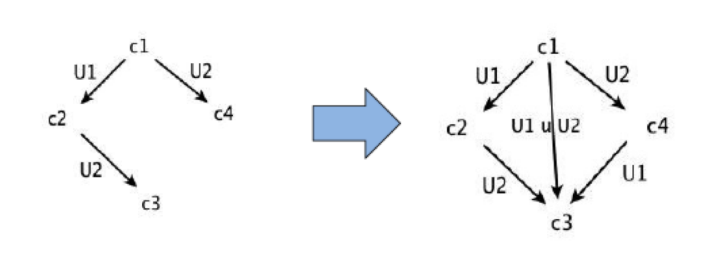
\includegraphics[width=0.5\textwidth]{img/reti/dp1.png}
                  \caption{Diamond property 1}
                  \label{fig:dp1}
              \end{figure}
        \item Supponiamo che $U_1 \cup U_2 \in U_{\Sigma}$ e che
              $U_1 \cap U_2 = \emptyset$, $U_1 \neq \emptyset, U_2 \neq \emptyset$.
              Allora se $c_1[U_1 \cup U_2 >c_3$ sicuramente $c_1[U_1 >$ e $c_1[U_2 >$
              e anche: $c_1[U_1 > c_2[U_2 >c_3$ e $c_1[U_2 > c_4[U_1 >c_3$. Segue
              quindi \ref{fig:dp2}.
              \begin{figure}[!ht]
                  \centering
                  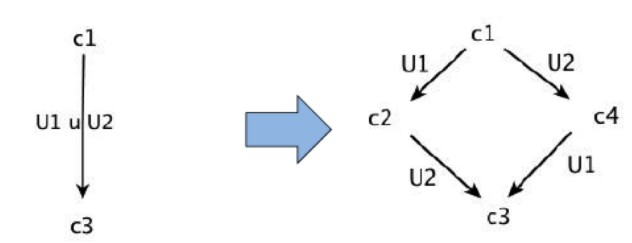
\includegraphics[width=0.5\textwidth]{img/reti/dp2.png}
                  \caption{Diamond property 2}
                  \label{fig:dp2}
              \end{figure}
    \end{enumerate}
\end{definizione}
Per la \textit{Diamond property}, nei sistemi elementari il grafo dei casi e il
grafo dei casi sequenziale sono \textit{sintatticamente equivalenti}, ovvero
possono essere ricavati l'uno dall'altro.

Questo implica il fatto che due sistemi elementari hanno grafi dei casi isomorfi
se e solo se hanno grafi dei casi sequenziale isomorfi.
\begin{definizione}[\textbf{Equivalenza tra sistemi}]
    Due sistemi $\Sigma_1$ e $\Sigma_2$ sono \textbf{equivalenti} se e solo se
    hanno grafi dei casi sequenziali, e quindi anche grafi dei casi, \textbf{isomorfi}.
\end{definizione}
\begin{definizione}[\textit{Problema della sintesi}]
    Dato un sistema di transizioni etichettato $A = (S, E,T,s_0)$, stabilire se
    esiste un sistema elementare $\Sigma = (B, E, F; c_{in})$ tale che: il suo
    grafo dei casi $SCG_{\Sigma}$ sia isomorfo ad $A$. E, in caso affermativo,
    costruire $\Sigma$.

    Questo problema è stato risolto usando la teoria delle regioni. Oltre a ciò,
    A dovrà soddisfare la Diamond property.
\end{definizione}
\begin{definizione}[\textbf{Contatto}]
    Sia $\Sigma = (B, E, F; c_{in})$ un sistema elementare, $e \in E$, $c \in C_{\Sigma}$
    allora $(e, c)$ è un \textbf{contatto} se e solo se:
    \begin{equation}
        ^{\bullet}e \subseteq c \ \land \ e^{\bullet} \cap c \neq \emptyset
    \end{equation}
\end{definizione}
\begin{definizione}[\textbf{Sistema senza contatti}]
    Un sistema elementare $\Sigma = (B, E, F; c_{in})$ è \textbf{senza contatti}
    se e solo se:
    \begin{equation}
        \forall e \in E, \ \forall c \in C_{\Sigma} \ \text{si ha} \ ^{\bullet}e \subseteq c \Rightarrow e^{\bullet} \cap c = \emptyset
    \end{equation}
\end{definizione}
È possibile trasformare un sistema elementare $\Sigma$ con contatti in un
sistema elementare $\Sigma_0$ che sia senza contatti aggiungendo a $\Sigma$ il
complemento di ogni condizione si ottiene un sistema $\Sigma_0$ con grafo dei
casi isomorfo a quello di $\Sigma$.
\begin{figure}[!ht]
    \centering
    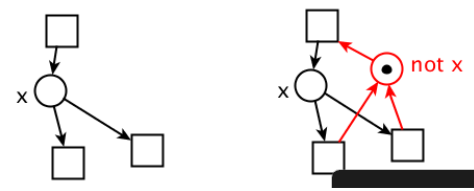
\includegraphics[width=0.5\textwidth]{img/reti/DelContatti.png}
    \caption{Complemento dell'operazione x.}
\end{figure}
Quindi se un sistema elementare $\Sigma$ è senza contatti allora per verificare
che un evento $e$ sia abilitato in un caso raggiungibile $c$ è sufficiente
verificare che le precondizioni di $e$ siano vere:
\begin{equation}
    c[e> \ \text{se e solo se} \ ^{\bullet} e \subseteq c
\end{equation}
\begin{definizione}[\textbf{Sequenza}]
    Sia $\Sigma = (B, E, F; c_{in})$ un sistema elementare, $c \in C_{\Sigma}$ $e_1, e_2, \in E$,
    allora $e_1$ ed $e_2$ sono in \textbf{sequenza} in $c$ se e solo se:
    \begin{equation}
        c[e_1 > \ \land \ \lnot c[e_2 > \ \land \ c[e_1e_2 > \ (c[e_1 > c'[e_2 >)
    \end{equation}
    \begin{figure}[!ht]
        \centering
        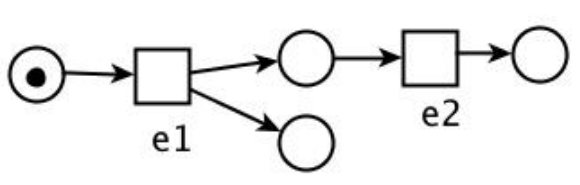
\includegraphics[width=0.5\textwidth]{img/reti/Seq.png}
        \caption{Rappresentazione della sequenza}
    \end{figure}
    In altre parole, è presente una relazione di dipendenza causale tra $e_1$ ed $e_2$
\end{definizione}
\begin{definizione}[\textbf{Concorrenti}]
    Sia $\Sigma = (B, E, F; c_{in})$ un sistema elementare, $c \in C_{\Sigma}$ $e_1, e_2, \in E$,
    allora $e_1$ ed $e_2$ sono \textbf{concorrenti} in $c$ se e solo se:
    \begin{equation}
        c[\{e_1, e_2\} >
    \end{equation}
    \begin{figure}[!ht]
        \centering
        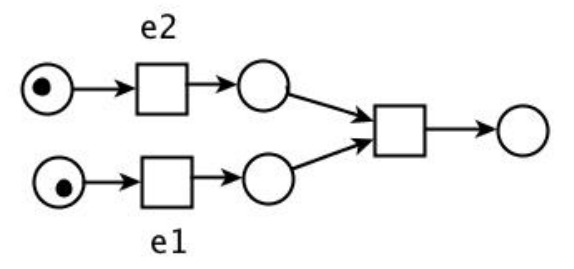
\includegraphics[width=0.5\textwidth]{img/reti/conc.png}
        \caption{Rappresentazione della concorrenza}
    \end{figure}
    In altre parole, se e sol se $e_1$ ed $e_2$ sono indipendenti ed entrambi
    abilitati in $c$.
\end{definizione}
\begin{definizione}[\textbf{Conflitto}]
    Sia $\Sigma = (B, E, F; c_{in})$ un sistema elementare,
    $c \in C_{\Sigma}$ $e_1, e_2, \in E$, allora $e_1$ ed $e_2$ sono in
    \textbf{conflitto} in $c$ se e solo se:
    \begin{equation}
        c[e_1 > \ \land \ c[e_2 > \ \land \ \lnot c[\{e_1, e_2\} >
    \end{equation}
    \begin{figure}[!ht]
        \centering
        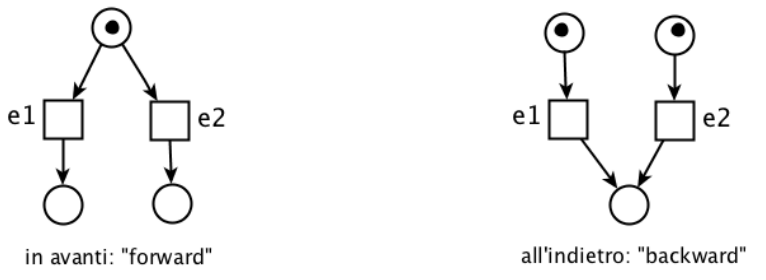
\includegraphics[width=0.5\textwidth]{img/reti/conf.png}
        \caption{Rappresentazione di un conflitto}
    \end{figure}
    In altre parole, sono entrambi abilitati ma l'occorrenza di uno disabilita
    l'altro.
\end{definizione}
Si definisce \textbf{confusione} quando non è possibile stabilire se è stato
risolto un conflitto.
\begin{definizione}[\textbf{Sottorete}]
    Siano $N = (B, E, F)$ e $N_1 = (B_1, E_1, F_1)$ due reti elementari. Diciamo che:
    \begin{itemize}
        \item $N_1 = (B_1, E_1, F_1)$ è \textbf{sottorete} di $N$ se e solo se:
              \begin{itemize}
                  \item $B_1 \subseteq B$
                  \item $E_1 \subseteq E$
                  \item $F_1 = F \cap [(B_1 \times E_1) \cup (E_1 \times B_1)]$
              \end{itemize}
        \item $N_1 = (B_1, E_1, F_1)$ è \textbf{sottorete generata da} $B_1$ se e solo se:
              \begin{itemize}
                  \item $B_1 \subseteq B$
                  \item $E_1 \subseteq ^{\bullet} B_1 \cup B_1^{\bullet}$
                  \item $F_1 = F \cap [(B_1 \times E_1) \cup (E_1 \times B_1)]$
              \end{itemize}
        \item $N_1 = (B_1, E_1, F_1)$ è \textbf{sottorete generata da} $E_1$ se e solo se:
              \begin{itemize}
                  \item $B_1 \subseteq ^{\bullet} E_1 \cup E_1^{\bullet}$
                  \item $E_1 \subseteq E$
                  \item $F_1 = F \cap [(B_1 \times E_1) \cup (E_1 \times B_1)]$
              \end{itemize}
    \end{itemize}
\end{definizione}
Data una rete $N = (B,E, F, c_0)$ questa può essere ottenuta componendo altre
reti di Petri. Si hanno in letteratura 3 modi principali:
\begin{enumerate}
    \item La composizione sincrona.
    \item La composizione asincrona.
    \item La composizione mista, tra sincrona e asincrona.
\end{enumerate}
\section{Processi non sequenziali}
\begin{definizione}[\textbf{Rete causale}]
    Definiamo $N = (B,E, F)$ come una \textbf{rete causale}, detta anche rete di
    occorrenze senza conflitti, se e solo se:
    \begin{itemize}
        \item $\forall b \in B: |^{\bullet}b| \leq 1 \land |b^{\bullet}| \leq 1$
              ovvero non si hanno conflitti; quindi, per ogni condizione si ha al più
              un pre-evento e un post evento. (Avendo quindi al più un arco entrante
              e al più uno uscente).
        \item $\forall x, y \in B \cup E: (x, y) \in F^{+} \Rightarrow (y, x \notin F^{+})$
              ovvero non si hanno cicli; quindi, presi due elementi collegati da una
              sequenza di archi orientati, avendo un cammino tra i due elementi ($F^{+}$
              è la chiusura transitiva della relazione $F$) non ho anche un cammino
              opposto tra i due.
        \item $\forall e \in E: \{x \in B \cup E | xF^{\ast}e\}$ è finito, ovvero
              si ha un numero finito di pre-elementi di un certo elemento.
    \end{itemize}
    Sono quindi reti che registrano un comportamento e quindi non si hanno
    conflitti (che in caso sono sciolti registrando solo quello che è effettivamente
    successo e non quello che potrebbe succedere). Si registra una run del sistema.
    Non si hanno nemmeno cicli perché ogni ripetizione dell'evento viene concatenata
    a quella prima.

    La rete può essere quindi si infinita ma è composta da un insieme di elementi
    finito che si ripete. In ogni caso il passato di un evento è finito e registrato,
    anche se nel complesso il comportamento è infinito “in avanti”. Con una rete
    causale si possono non distinguere più condizioni ed eventi.
\end{definizione}
Ad una rete causale è possibile associare un \textbf{ordine parziale}:
\begin{equation}
    (X, \leq) = (B \cup E, F^{\ast})
\end{equation}
Dicendo che un elemento “è minore” di un altro se esiste un cammino orientato
dall'uno all'altro.
\begin{definizione}
    Data una rete causale $N = (B,E, F)$ e dato un ordine parziale $(X, \leq)$
    con $X = B \cup E$ si ha che si può interpretare la relazione d'ordine come
    indipendenza o dipendenza causale, ovvero presi $x, y \in X$ come elementi
    che occorrono nella storia di $X = B \cup E$ si hanno le seguenti diciture:
    \begin{itemize}
        \item $x \leq y$ (avendo un cammino da $x$ a $y$) corrisponde a $x$ causa
              $y$, ovvero si ha una relazione di dipendenza causale tra i due.
        \item $x \ \textbf{li} \ y$ indica che $x \leq y \lor y \leq x$ e quindi
              corrisponde a $x$ e $y$ sono causalmente dipendenti. Si ha che \textbf{li}
              può venire letto come linea ($x$ in linea con $y$) avendo che uno dei
              due precede l'altro.
        \item $x \textbf{co} \ y$ indica che: $\lnot(x < y)\  \land  \ \lnot (y < x)$
              e quindi corrisponde a $x$ e $y$ sono \textbf{causalmente indipendenti},
              avendo che i due elementi non si precedono a vicenda, non avendo ordine
              tra loro. Si ha che \textbf{co} sta per concurrency.
    \end{itemize}
\end{definizione}
\begin{definizione}
    Data una rete causale $N = (B,E, F)$ e dato un ordine parziale $(X, \leq)$
    con $X = B \cup E$ definiamo:
    \begin{equation}
        C \subseteq X
    \end{equation}
    come:
    \begin{itemize}
        \item \textbf{co-set} se e solo se $\forall x, y \in C$: $x \ \textbf{co} \ y$,
              quindi $C$ è una clique della relazione \textbf{co}.
        \item \textbf{taglio} se e solo se $C$ è un \textbf{co-set} massimale
              (tutti gli elementi nel taglio sono in relazione \textbf{co})
    \end{itemize}
    Definiamo $C$ come \textbf{co-set} massimale se e solo se $\forall y \in X \cap C$
    si ha che:
    \begin{equation}
        \exists c \in C: y \not\textbf{co} \ c
    \end{equation}
    Quindi in $C$ definito o come \textbf{co-set} o come \textbf{taglio} si ha
    che vale la transitività. Definiamo:
    \begin{equation}
        L \subseteq X
    \end{equation}
    come:
    \begin{itemize}
        \item \textbf{li-set} se e solo se $\forall x, y \in L: \ x \ \textbf{li} \ y$
        \item \textbf{linea} se e solo se $L$ è un \textbf{li-set} massimale.
    \end{itemize}
    Definiamo $L$ come \textbf{li-set} massimale se e solo se $\forall y \in X \backslash L$ si ha che:
    \begin{equation}
        \exists l \in L: \ y \not\textbf{li}  \ l
    \end{equation}
    Si ha quindi che:
    \begin{itemize}
        \item In un \textbf{co-set} la relazione \textbf{co} è transitiva.
        \item In un \textbf{li-set} la relazione \textbf{li} è transitiva.
    \end{itemize}
    Tagli e linee possono essere fatti sia di condizioni che di eventi.
\end{definizione}
Un taglio $C \subseteq X$ è detto $B$-taglio se $C \subseteq B$.

I tagli fatti di sole condizioni rappresentano casi raggiungibili dal sistema.

Una rete causale, quindi, registra il comportamento di un sistema elementare. Si
hanno quindi, con i tagli, possibili osservazioni di configurazioni possibili
nella storia del sistema.
\begin{definizione}
    Grazie alle reti causali, preso un elemento $x \in X$, possiamo definire:
    \begin{itemize}
        \item $\textbf{past}(x)$, ovvero il passato dell'elemento, tutti gli
              elementi in relazione $\leq$ di $x$.
        \item $\textbf{future}(x)$, ovvero il futuro dell'elemento, tutti gli
              elementi in relazione $\geq$ di $x$.
    \end{itemize}
    Gli elementi nell'anti-cono sono in relazione \textbf{co} con $x$ e quindi
    possono essere concorrenti.
\end{definizione}
\begin{definizione}[\textbf{k-densità}]
    $N = (B, E, F)$ rete causale, $(X = (B \cup E), \leq)$ ordine parziale. Si
    ha che $N$ è \textbf{$k-$densa} se e solo se:
    \begin{equation}
        \forall h \in Linee(N), \ \forall c \in Tagli(N): \ |h \cap c| = 1
    \end{equation}
    dove $Linee(N)$ e $Tagli(N)$ sono gli insiemi delle linee e dei tagli di $N$.
\end{definizione}
\begin{nota}
    Se la rete causale $N$ è finita allora $N$ è anche $K-$densa.
\end{nota}
\begin{figure}[!ht]
    \centering
    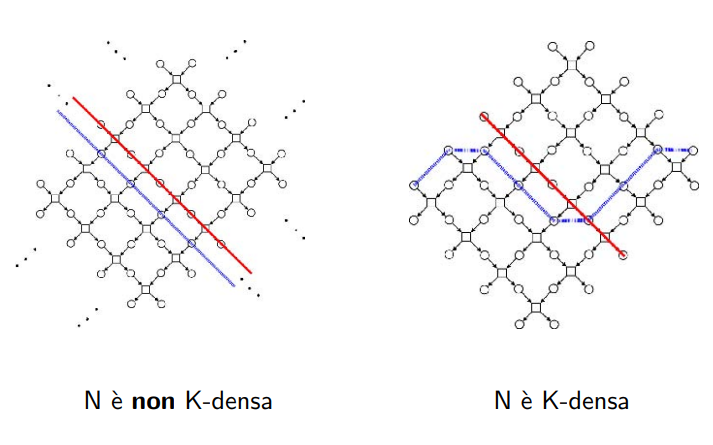
\includegraphics[width=0.7\textwidth]{img/reti/kdensa.png}
    \caption{Esempio di rete $K$-densa}
\end{figure}
\begin{definizione}[\textbf{Processi non sequenziali}]
    Sia $\Sigma = (S, T, F, c_{in})$ un sistema elementare senza contatti e finito,
    ovvero con $S \cup T$ finito.

    $\langle N = (B, E, F), \phi \rangle$ è un processo non sequenziale si $\Sigma$
    se e solo se:
    \begin{itemize}
        \item $(B, E, F)$ è una rete causale nella quale si ammettono condizioni
              isolate.
        \item $\phi: B \cup E \to S \cup T$ è una mappa tale che:
              \begin{enumerate}
                  \item $\phi(B) \subseteq S, \ \phi(E) \subseteq T$
                  \item $\forall x_1, x_2 \in B \cup E: \ \phi(x_1) = \phi(x_2) \Rightarrow (x_1 \leq x_2) \ \lor \ (x_2 \leq x_1)$
                  \item $\forall e \in E: \ \phi(^{\bullet}e) = ^{\bullet}\phi(e) \ \land \ \phi(e^{\bullet}) = \phi(e)^{\bullet}$
                  \item $\phi(Min(N)) = c_{in}$ dove
                        $Min(N) = \{x \in B \cup E | \not\exists y: \ (y, x) \in F\}$
                        ovvero non hanno un arco entrante, sono gli stati locali iniziali.
              \end{enumerate}
    \end{itemize}
\end{definizione}
Se $\langle N = (B, E, F); \phi \rangle$ è un processo non sequenziale di
$\Sigma = (S, T, F, c_{in})$ sistema elementare finito e senza contatti allora:
\begin{itemize}
    \item $N = (B, E, F)$ è $K$-densa
    \item $\forall K \in B$, $K\ B$-taglio di $N$ è tale che: $K$ è finito e
          $\exists c \in C_{\Sigma}: \ \phi(K) = c$
\end{itemize}
\subsection{Reti di Occorrenze}
\begin{definizione}[\textbf{Rete di occorrenze}]
    $N = (B, E, F)$ è una \textbf{rete di occorrenze} se e solo se:
    \begin{itemize}
        \item $\forall b \in B: \ | ^{\bullet}| \leq 1$ sono presenti dei conflitti
              solo in avanti.
        \item $\forall x, y \in B \cup E: \ (x, y) \in F^{+} \Rightarrow (y, x) \notin F^{+}$
              non ci sono cicli
        \item $\forall e \in E: \{x \in B \cup E| \ xF^{\ast} e \}$ è finito
        \item La relazione di conflitto $\#$ non è riflessiva. La relazione di
              conflitto è definita come:
              \begin{equation}
                  \# \subseteq X \times X \ \text{dove} \ X = B \cup E \ \text{è definita come}: \\
                  x\#y \ \text{se e solo se} \ \exists e_1, e_2 \in E: \ ^{\bullet} e_1 \cap ^{\bullet} e_2 \neq \emptyset \ \land e_1 \leq x \ \land \ e_2 \leq y
              \end{equation}
    \end{itemize}
\end{definizione}
In queste reti è ancora possibile associare a $N$ un ordine parziale $(X, \leq) = (B \cup E, F^{\ast})$
\begin{definizione}[\textbf{Processo ramificato}]
    Sia $\Sigma = (S,T, F, c_{in})$ un sistema elementare senza contatti e finito.
    $\langle N = (B, E, F); \phi \rangle$ è un \textbf{processo ramificato} di $\Sigma$
    se e solo se:
    \begin{itemize}
        \item $(B, E, F)$ è una rete di occorrenze (si ammettono condizioni isolate)
        \item $\phi: B \cup E \to S \cup T$ è una mappa:
              \begin{enumerate}
                  \item $\phi(B) \subseteq S, \ \phi(E) \subseteq T$
                  \item $\forall e_1, e_2 \in E: \ ( ^{\bullet} e_1 =  ^{\bullet} e_2 \ \land \ \phi(e_1) = \phi(e_2)) \Rightarrow e_1 = e_2$
                  \item $\forall e \in E$ : la restrizione di $\phi$ a $^{\bullet} e$
                        è una biiezione tra $^{\bullet} e \ \text{e} \ ^{\bullet} \phi(e)$
                        e la restrizione di $\phi$ a $^{\bullet}$ è una biiezione tra
                        $e^{\bullet} \ \text{e} \ \phi(e)^{\bullet}$
                  \item La restrizione di $\phi$ a $Min(N)$ è una biiezione tra
                        $Min(N)$ e $c_{in}$.
              \end{enumerate}
    \end{itemize}
\end{definizione}
La proprietà 2 e 3 delle reti causali in and tra loro implicano la proprietà 3
delle reti di occorrenze. Un ragionamento analogo può essere fatto per le proprietà
2 e 4 delle reti causali, le quali in and implicano la proprietà 4 delle reti
di occorrenza.
\begin{nota}
    Un processo non sequenziale può essere definito anche richiedendo che $\phi$
    soddisfi: (1),(2),(3') e (4'), dove 3' e 4' implicano le proprietà 3 e 4
    delle reti di occorrenza.
\end{nota}
\begin{definizione}[\textbf{Prefisso}]
    Sia $\Sigma = (S,T, F, c_{in})$ un sistema elementare finito e senza contatti
    e siano $\Pi_1 = \langle N_1; \phi_1 \rangle$, $\Pi_2 = \langle N_2; \phi_2 \rangle$
    processi ramificati di $\Sigma$.

    Allora $\Pi_1 = \langle N_1; \phi_1 \rangle$ è un \textbf{prefisso} di
    $\Pi_2 = \langle N_2; \phi_2 \rangle$ se e solo se $N_1$ è una sottorete di
    $N_2$ e $\phi_{2|N_1} = \phi_1$ ($\phi_2$ ”ristretto” a $N_1$ è uguale a $\phi_1$).
\end{definizione}
\begin{definizione}
    $\Sigma$ ammette un unico processo ramificato che è massimale rispetto alla
    relazione di prefisso tra processi. Tale processo massimale è chiamato
    \textbf{unfolding} di $\Sigma$, denotato $Unf (\Sigma)$.
\end{definizione}
\begin{definizione}
    Un processo non sequenziale è un processo ramificato $\Pi = \langle N; \phi \rangle$
    tale che $N$ sia una rete causale (senza conflitti), tale processo è chiamato
    anche \textbf{corsa} (\textbf{run}).
\end{definizione}
\begin{osservazione}
    Inoltre, ogni processo non sequenziale di $\Sigma$ è un prefisso dell'unfolding
    $Unf (\Sigma)$.
\end{osservazione}
\section{Sistemi elementari - reti P/T- Reti ad alto livello}
Se dovessimo usare le reti elementari per modellare sistemi veri, avremmo
un'esplosione di condizioni ed eventi. Una rappresentazione più compatta è data
dalle \textbf{reti Posti e Transizioni} che utilizzano, invece delle condizioni
booleane dei sistemi elementari, dei contatori.
\begin{definizione}[\textbf{Sistema Posti e Transizioni}]
    Formalmente un sistema posti e transizioni è definito come:
    \begin{equation}
        \sigma = (S, T, F, K, W, M_0)
    \end{equation}
    dove:
    \begin{itemize}
        \item $(S, T, F)$ è una rete.
        \item $K: S \to \mathbb{N}^+ \cup {\infty}$ è la funzione che assegna ai
              posti le capacità
        \item $W: F \to \mathbb{N}$ è la funzione peso degli archi
        \item $M_0: S \to \mathbb{N}: \forall s \in S$ $M_0(s) \leq K(s)$ è la
              marcatura iniziale. È importante osservare che il numero di marche è sempre
              minore o uguale alla capacità del posto
    \end{itemize}
\end{definizione}
Ad esempio, pensiamo ad un buffer a due posizioni, nei sistemi elementari avremmo
due condizioni con due eventi deposita e preleva. Nei sistemi P/T possiamo usare
un contatore come fosse un'unica condizione. Chiaramente si perde dell'informazione,
in particolare non sappiamo più in quale posizione del buffer il produttore
deposita e da quale posizione il consumatore consuma.

Questa tipologia di reti mi permette di definire degli archi pesati, archi con
associato un numero, che abilitino o meno le transizioni.

Le reti ad alto livello, anche dette \textbf{reti colorate}, permettono di
ristabilire l'informazione persa con le reti Posti e transizioni assegnando una
struttura dati alle marche. Addirittura, una marca potrebbe rappresentare un
processo a sé stante.
\begin{definizione}[\textbf{Regola di scatto}]
    \begin{equation}
        M[t > \ \text{se e solo se} \ \forall s \in S \ M(s) \geq W(s, t) \ \land \ M(s) \ \text{è} \ W(t, s) \leq K(s)
    \end{equation}
    \begin{equation}
        M[t > M' \ \text{se e solo se} \ M[t > \ \land \ \forall s \in S \ M'(s) = M(s) - W(s, t) + W(t, s)
    \end{equation}
\end{definizione}
Anche qui, come nei sistemi elementari si può costruire l'insieme delle marcature
raggiungibili e il relativo grafo di raggiungibilità. Generalmente in queste reti
la Diamond property non è più valida.
\begin{definizione}[\textbf{Reti marcate}]
    Un sistema Posti e transizione è una rete marcata se non ha vincoli sulla
    capacità dei posti e ha tutti gli archi di peso unitario.
\end{definizione}
Una rete marcata è \textbf{safe} se comunque evolva il comportamento avremmo in
ogni posto sempre al più una marca, i posti hanno quindi $0$ o $1$ marca e possiamo
interpretarli di nuovo come condizioni booleane. L'unica differenza con le reti
elementari è che nelle reti safe i cappi sono abilitati, mentre nelle reti
elementari questo non succede.

Se eliminiamo i cappi dalle reti marcate safe, otteniamo il corrispettivo di un
sistema elementare puro.

\textbf{Da completare perché mancano le slide}
\chapter{Dimostrazioni di correttezza}
\section{Logica proposizionale}
Nella logica proposizionale, dal punto di vista teorico, il significato di una formula è rappresentato dal suo valore di verità.

Una volta definite sintassi e semantica, possiamo usare una logica per costruire delle dimostrazioni; aver definito una semantica non vuol dire che di fronte ad una formula si è in grado di dire subito se sia valida o meno, dunque con la logica si sviluppa un metodo di dimostrazione e si cerca, in un numero finito di passi, di dimostrare la validità di una certa formula.

Un esempio, legato alla logica dell'aritmetica, è la formula che dice che per ogni numero primo, esiste sempre un numero primo più grande di esso; questa formula non è verificabile sperimentalmente essendo in numeri infiniti e va quindi dimostrata in altri modi.

Per ogni logica bisogna quindi definire un apparato deduttivo, cioè un insieme di regole di \textbf{inferenza}. Una regola di inferenza è una regola che dice "se hai già dimostrato queste premesse, allora puoi dedurre questa formula".

\subsection{Sintassi}
Passiamo ora al caso specifico della logica proposizionale che ci servirà per le dimostrazioni di correttezza.

Per costruire il linguaggio avremmo bisogno di:
\begin{itemize}
    \item $PA = \{p_1, \dots, pi, \dots\}$ sono le proposizioni atomiche.
    \item $\bot, \ \top$ sono le costanti logiche, rappresentano formule o sempre false o sempre vere.
    \item $\lnot, \ \land, \ \lor, \ \to, \ \leftrightarrow$ sono i connettivi logici, utilizzati per creare formule complesse.
    \item $(, \ )$ sono i demilitatori, utilizzati per la creazione di formule complesse.
\end{itemize}
Adesso dobbiamo definire la grammatica della logica proposizionale, per fare ciò si utilizza una definizione induttiva.
\begin{definizione}[\textbf{Formule ben formate}]
    Definiamo l'insieme delle formule ben formate $F_p$ come:
    \begin{itemize}
        \item $\bot, \ \top \in F_p$ le costanti logiche sono delle formule ben formate.
        \item $\forall p_i \in PA, \ p_i \in F_p$ le proposizioni atomiche sono formule ben formate.
        \item Se $A, B \ in F_p$ allora:
        \begin{equation}
            (\lnot A), \ (A \land B), \ (A \lor B), \ (A \to B), \ (A \leftrightarrow B) \ \in F_p
        \end{equation}
        \item Nient'altro è una formula ben formata.
    \end{itemize}
\end{definizione}
Le formule atomiche rappresentano delle relazioni tra le variabili e le costanti oppure relazioni tra le variabili.
\subsection{Semantica}
Siamo ora interessati a conoscere il valore di una formula scritta attraverso la logica proposizionale. Il \textbf{valore di verità} di una formula dipende dai valori di verità delle sue proposizioni atomiche.

Il punto di partenza è quindi stabilire quali proposizioni atomiche sono da considerare vere. Questo si può fare formalmente definendo una \textbf{funzione di valutazione}:
\begin{equation}
    v: PA \to \{0, 1\}
\end{equation}

I connettivi della Logica Proposizionale hanno i seguenti valori di verità:
\begin{equation}
    \begin{array}{ccccccc}
    \toprule
    \text{A} & \text{B} & A \land B & A \lor B & \neg A & A \to B & A \longleftrightarrow B \\
    \midrule
    F & F & F & F & T & T & T \\
    F & T & F & T & T & T & F \\
    T & F & F & T & F & F & F \\
    T & T & T & T & F & T & T \\
    \bottomrule
  \end{array}
\end{equation}
Questa funzione di valutazione può essere estesa induttivamente ad una funzione definita su tutte le formule ben formate, tale funzione prende il nome di \textbf{funzione di interpretazione} ed è definita come:
\begin{equation}
    I_v: F_p \to \{0, 1\}
\end{equation}
\begin{enumerate}
    \item $I_v (\bot) = 0$ e $I_v (\top) = 1$ le costanti logiche hanno valore di verità definito.
    \item $\forall p_i \in PA \ I_v(p_i) = v(p_i)$ l'interpretazione di una preposizione atomica è data dal suo valore di verità.
    \item Passo induttivo:
    \begin{equation}
        \begin{array}{cc}
           I_v(\lnot A) = 1 - I_v(A) & \\ 
           I_v(A \lor B) = 1 & \text{se e solo se} \ I_v(A) = 1 \ \text{o} \ I_v(B) = 1 \\
           \dots & \\
           I_v(A \to B) = 1 & \text{se e solo se} \ I_v(A) = 0 \ \text{o} \ I_v(B) = 1 
        \end{array}
    \end{equation}
\end{enumerate}
Vediamo ora un'po di terminologia:
\begin{itemize}
    \item $A$ è \textbf{soddisfatta} da $I_v$ se $I_v(A) = 1$.
    \item $A$ è \textbf{soddisfacibile} se esiste $I_v$ tale che $I_v(A) = 1$.
    \item $A$ è una \textbf{tautlogia} se $I_v(A) = 1$ per ogni $I_v$
    \item $A$ è una \textbf{contraddizione} se $I_v(A) = 0$ per ogni $I_v$
\end{itemize}
\begin{definizione}[\textbf{Logicamente equivalenti}]
    Due formule ben formate $A$ e $B$ sono logicamente equivalenti, indicato con $A \equiv B$, se e solo se:
    \begin{equation}
        I_v(A) = I_v(B) \ \ \forall I_v
    \end{equation}
\end{definizione}
\begin{definizione}\textbf{[Modello]}
    Definiamo ora i modelli, ovvero delle interpretazioni delle proposizioni atomiche, cioè una scelta di valori di verità per tutte le proposizioni atomiche.
    
    Un modello è un sottoinsieme delle proposizioni atomiche $M \subseteq PA$ a cui è associata un'interpretazione definita come $I_M: F_p \to \{0, 1\}$ tale che:
    \begin{equation}
        I_M(p_i) = 1 \ \text{se e solo se} \ p_i \in M
    \end{equation}
    Possiamo indicare la relazione tra modelli e formule come:
    \begin{equation}
        M \models A
    \end{equation}
    la quale si può leggere come $M$ modella $A$ oppure come $A$ è soddisfatta in $M$. Quindi scriveremo $M \models A$ se $A$ risulta vera per la scelta particolare di $M$.
\end{definizione}
\begin{definizione}
     Se $M \models A$ per tutti gli $M$, allora $A$ è una tautologia e si indica $\models A$.
\end{definizione}
\begin{definizione}
    Se $M \models A$ per qualche $M$, allora $A$ è soddisfacibile.
\end{definizione}
\begin{definizione}
    Se $M \models A$ non è soddisfatta da nessun $M$, allora $A$ è in soddisfacibile.
\end{definizione}
Definizione 6. 
Definizione 7. 
\subsection{Apparato deduttivo}
Possiamo ora rappresentare l'apparato deduttivo della logica proposizionale. Esso è composto da \textbf{regole di inferenza} scritte in questo modo:
\begin{equation}
    \frac{A_1, \dots, A_n}{B}
\end{equation}
dove $A_i \in F_p$ sono le premesse, mentre $B \in F_p$ è la conclusione.

Alcune regole di inferenza sono ad esempio:
\begin{itemize}
    \item Se ho dimostrato che $A_1$ e $A_2$ sono vere, sarà vera anche $A_1 \land A_2$: 
    \begin{equation}
        \frac{A_1 \ \ A_2}{A_1 \land A_2}
    \end{equation}
        \item Se ho dimostrato che $A_1 \land A_2$ è vera, sarà vera anche $A_1$: 
    \begin{equation}
        \frac{A_1 \land A_2}{A_1}
    \end{equation}
    \item Modus Ponens:
    \begin{equation}
        \frac{A \ \ A \to B}{B}
    \end{equation}
    \item Modus Tollens:
    \begin{equation}
        \frac{A \to B \ \ \lnot B}{\lnot A}
    \end{equation}
\end{itemize}

Le regole di inferenza sono la base da cui è possibile costruire le dimostrazioni.
\begin{definizione}[\textbf{Dimostrazione}]
    Una dimostrazione è definita come una catena di regole $A_1,\dots, A_n \vdash B$, ovvero da $A_1, \dots, A_n$ si deriva $B$.  
\end{definizione}
Abbiamo ora due nozioni distinte:
\begin{itemize}
    \item La validità in un modello $\models$
    \item La derivabilità $\vdash$ introdotta perché in generale non siamo in grado di decidere direttamente la nozione semantica di validità e quindi cerchiamo di dimostrare una cosa.
\end{itemize}
\begin{teorema}[\textbf{(Validità, Correttezza)}]
    Se $A_1, \dots, A_n \vdash B$ allora $A_1, \dots, A_n \models B$. Ovvero, se riusciamo a derivare $B$ da $A_1, \dots, A_n$ in ogni modello in cui sono vere $A_1, \dots, A_n$ allora è vera anche $B$.
\end{teorema}
Questo teorema ci dice che abbiamo scelto bene le regole di inferenza e che queste non ci permettono di derivare cose non vere. Se questo teorema è valido, la logica è corretta.
\begin{teorema}[\textbf{Completezza}]
    Se $A_1, \dots, A_n \models B$ allora $A_1, \dots, A_n \vdash B$, ovvero se in ogni modello in cui sono vere $A_1, \dots, A_n$ ed è vera anche $B$, si può derivare $B$ da $A_1, \dots, A_n$.
\end{teorema}
Questo teorema ci dice che possiamo dimostrare tutto ciò che è vero. Se questo teorema è valido, la logica è completa.
\section{Logica di Hoare}
Questa logica si può vedere come costruita su due livelli diversi poiché permette di stabilire e definire il criterio di correttezza per un dato programma. In particolare, definisce questa correttezza tramite le definizioni di precondizioni e postcondizioni che sono delle formule della logica proposizionale.
\subsection{Primo livello}
Al primo livello avremmo le proposizioni atomiche definite come relazioni fra le variabili del programma, tra queste relazioni possiamo trovare anche relazioni tra le variabili e le costanti.

Per dare una semantica, alle varie proposizioni atomiche definiamo la nozione di \textbf{stato della memoria}.
\begin{definizione}[\textbf{Stato di memoria}]
    Sia $V$ l'insieme delle variabili del programma, definiamo uno stato della memoria come una fotografia della memoria del programma in un certo istante.

    Possiamo definire più formalmente quest'idea di stato della memoria come una funzione definita dall'insieme delle variabili ai numeri interi che assegna un valore ad ogni variabile.
    \begin{equation}
        \sigma: V \to \mathbb{Z}
    \end{equation}
    Diremo quindi che la formula $\alpha$ è vera in $\sigma$ scrivendo $\sigma \models \alpha$
\end{definizione}
\subsection{Secondo livello}
Le formule della logica di Hoare sono costruite tramite delle triple che prendono il nome di triple di Hoare, le quali sono definite come: 
\begin{equation}
    \{\alpha\} \ C \ \{\beta\}
\end{equation}
dove:
\begin{itemize}
    \item $\{\alpha\}$ è una formula che rappresenta le pre-cndizioni.
    \item $C$ rappresenta un programma o un comando
    \item $\{\beta\}$ è una formula che rappresenta le post-condizioni.
\end{itemize}
Le triple di Hoare si leggono come segue:
\begin{center}
    Se il comando $C$ viene eseguito a partire da uno stato della memoria nel quale $\alpha$ è vera, allora l'esecuzione termina e nello stato finale $\beta$ è vera.
\end{center}
\subsection{Linguaggio}
Definiamo ora il linguaggio che useremo con le triple di Hoare:
\begin{itemize}
    \item Espressioni aritmetiche $E$ definite come:
    \begin{equation}
        \forall z \in \mathbb{Z} \ z \in E \ \land \ \forall e_1, e_2 \in E \ (e_1 + e_2), (e_1 - e_2), -e_1, (e_1 \ast e_2), (e_1 / e_2), (e_1 \% e_2) \in E
    \end{equation}
    \item Espressioni logiche $B$ definite come:
    \item Comandi $C$ definiti come:
    \begin{itemize}
        \item Assegnamento $x := e \ \in C$ dove $v$ è una variabile ed $e$ è un espressione aritmetica.
        \item Operatore di sequenza $C, D \ \in C $ dove $C$ e $D$ sono dei comandi.
        \item Operatore di scelta $\text{if} \ B \ \text{then} \ C \ \text{else} \ D \ \text{endif} \ \in C$ dove $B$ è un espressione logica, mentre $C, D$ è sono dei comandi.
        \item Operatore di iterazione $\text{while} \ B \ \text{do} \ C \ \text{endwhile}$ dove $B \in C$ è un espressione logica e $C$ è un comando.
        \item $\text{skip} \in C$ questa istruzione non modifica la memoria.
    \end{itemize}
\end{itemize}

Una tripla di Hoare rappresenta un criterio di correttezza del programma, la sua regola di derivazione è definita come:
\begin{equation}
    \frac{T_1, \dots, T_m, f_1, \dots, f_n}{T}
\end{equation}
dove al numeratore sono specificate le premesse che possano contenere sia triple $T_i$ che formule ben formate $f_i$, mentre al denominatore troviamo la conclusione che è una tripla $T$.

Vediamo ora come definire le regole di derivazione per i comandi introdotti:
\begin{enumerate}
    \item Per il comando \textbf{skip} definiamo la seguente regola di derivazione:
    \begin{equation}
        \frac{}{\{p\} \text{ skip } \{p\}}
    \end{equation}
    in questo caso la premessa è vuota e, visto che con questa operazione non modifico lo stato della memoria, le pre-condizioni e le post-condizioni sono le stesse.
    \item Per il comando \textbf{sequenza} definiamo la seguente regola di derivazione:
    \begin{equation}
        \frac{\{p\} \text{ C } \{p'\} \ \ \{p'\} \text{ D } \{q\}}{\{p\} \text{ C; D } \{p\}}
    \end{equation}
    se le post-condizioni di C  e le pre-condizioni di D sono le stesse posso mettere in sequenza i comandi ottenendo lo stesso risultato.
        \item Per il comando \textbf{scelta} definiamo la seguente regola di derivazione:
    \begin{equation}
        \frac{\{p \land B\} \text{ C } \{q\} \ \ \{p \land \lnot B\} \text{ D } \{q\}}{\{p\} \text{ if B then C else D endif } \{q\}}
    \end{equation}
    Se dimostriamo che
    \begin{itemize}
        \item Eseguendo C da uno stato dove vale la precondizione $p$ e vale anche la condizione $B$ al termine dell'esecuzione vale $q$.
        \item Eseguendo $C$ da uno stato dove vale $p$ ma non vale $B$ arriviamo comunque ad uno stato dove vale $q$.
    \end{itemize}
    Possiamo derivare la regola della scelta dove prima dell'esecuzione dell'$if$ vale $p$ mentre dopo vale $q$.
    \item Per il comando \textbf{implicazione} definiamo la seguente regola di derivazione:
    \begin{equation}
        \frac{p \to p' \ \ \{p'\} \text{ C } \{q\}}{\{p\} \text{ C } \{q\}}
    \end{equation}
    inoltre:
    \begin{equation}
        \frac{\{p\} \text{ C } \{q\} \ \ q \to q'}{\{p\} \text{ C } \{q'\}}
    \end{equation}
    Generalizzando possiamo dire che se abbiamo dimostrato una tripla e osserviamo una condizione che implica la precondizione della tripla, possiamo derivare la tripla con la condizione osservata al posto della precondizione. Discorso analogo è valido anche per la post-condizione.
    \item Per il comando \textbf{assegnamento} definiamo la seguente regola di derivazione:
    \begin{equation}
        \frac{}{\{q[E/q]\} \text{ x } := \text{ E }\{q\}}
    \end{equation}
    dove con $q[E / x]$ indico il fatto che sostituisco ogni occorrenza di $x$ in $q$ con $E$.
    \item Per il comando \textbf{iterazione} (correttezza parziale) definiamo la seguente regola di derivazione:
    \begin{equation}
        \frac{\{inv \land B\} \text{ C } \{inv\}}{\{inv\} \text{ while B do C endwhile } \{inv \land \lnot B\}}
    \end{equation}
    l'idea per le istruzioni iterative è di trovare una formula che sia invariante rispetto al blocco dell'istruzione iterativa. Se troviamo un'invariante possiamo dire che se questa formula è vera all'inizio dell'istruzione iterativa, lo sarà anche alla fine e in più possiamo dire che al termine del blocco iterativo vale anche la negazione della condizione di ciclo.
    
    In generale, avendo un'istruzione $W = \text{ while B do C endwhile }$, se deriviamo $\vdash \{p \land B\} C \{p\}$, allora possiamo dire che $p$ è invariante rispetto a $W$.
    
    Data un'istruzione iterativa, non c'è un solo invariante. Ad esempio, $True$ è invariante per ogni istruzione iterativa. Generalmente ci interessano gli invarianti utili alla dimostrazione in corso. Nella pratica, le istruzioni iterative sono inserite in programmi, di conseguenza la scelta dell'invariante dipende dal contesto e si abbina alla regola dell'implicazione.
    
    A volte l'invariante non è assoluto, ma lo diventa aggiungendoci la condizione di ciclo. L'invariante in genere è violata guardando lo stato della memoria durante l'esecuzione del blocco, ma viene ripristinata al termine del blocco.
\end{enumerate}

\begin{definizione}[\textbf{Invariante di un ciclo}]
    Possiamo definire l'\textbf{invariante di un ciclo} come una formula che se risulta vera all'inizio di un iterazione è vera anche alla fine di essa.
\end{definizione}

La logica di Hoare è una logica \textbf{corretta}, ovvero vale:
\begin{equation}
    \vdash \to \models
\end{equation}
questo significa che tutte le triple che riusciamo a derivare sono sicuramente delle triple valide. Inoltre, è anche \textbf{completa} (relativamente):
\begin{equation}
    \models \to \vdash
\end{equation}
tutto ciò che è valido è derivabile. Tuttavia è una completezza relativa a causa dell'incompletezza dell'aritmetica: potrebbe succedere di dover dimostrare una proprietà aritmetica che però è indimostrabile (caso molto remoto).

Come notazione usiamo che:
\begin{equation}
    \vdash \{p\} \text{ C } \{q\}
\end{equation}
dove $\vdash$ segnala che la tripla è stata dimostrata/derivabile con le regole di derivazione (si parla quindi di sintassi, viene infatti ignorato il significato ma si cerca solo di applicare le regole, ottenendo al conclusione come risultato di
una catena di regole).

Usiamo anche:
\begin{equation}
    \models \{p\} \text{ C } \{q\}
\end{equation}
dove $\models$ indica che la tripla è vera (si parla quindi di semantica, riferendosi al significato).

Dato che si ha completezza e correttezza dell’apparato deduttivo si ha hanno due situazioni.
\begin{itemize}
    \item ogni tripla derivabile è anche vera in qualsiasi interpretazione.
    \item ogni tripla vera vorremmo fosse anche derivabile e il discorso verrà approfondito in seguito per la logica di Hoare
\end{itemize}
$\vdash$ può avere a pedice una sigla per la regola rappresentata.
\subsection{Correttezza totale}
Vogliamo ora analizzare la correttezza totale dell'istruzione while, ovvero si vuole verificare anche la terminazione del ciclo:
\begin{equation}
    \{p\} \ \text{while B do C endwhile} \ \{q\} 
\end{equation}
\begin{definizione}[\textbf{Correttezza parziale}]
    Definiamo la \textbf{correttezza parziale} come: "Se si esegue $W$ a partire da uno stato in cui vale $p$ e l'esecuzione termina, nello stato finale vale $q$" $$\stackrel{parz}{\vdash} \{p\} C_1 \{q\}$$
\end{definizione}
\begin{definizione}[\textbf{Correttezza totale}]
    Definiamo la \textbf{correttezza totale} come: "Se si esegue $W$ a partire da uno stato in cui vale $p$, l'esecuzione termina e nello stato finale vale $q$" $$\stackrel{tot}{\vdash} \{p\} C_1 \{q\}$$
\end{definizione}
Vediamo ora una tecnica per dimostrare la correttezza totale. Supponiamo che $E$ sia un'espressione aritmetica nella quale compaiono variabili del programma, costanti numeriche e operazioni aritmetiche, e che $inv$ sia un invariante di ciclo per $W$, scelti in modo che:
\begin{enumerate}
    \item $inv \to E \geq 0$
    \item $\stackrel{tot}{\vdash} \{inv \land B \land E = k > 0\} \ C \ \{inv \land E < k\}$
\end{enumerate}
Allora:
\begin{equation}
    \stackrel{tot}{\vdash} \{inv\} \ W \ \{inv \land \lnot B\}
\end{equation}
\begin{nota}
    $E$ non è una formula logica, ma $E \geq 0$ è una formula logica. Lo $0$ in $E \geq 0$ può essere sostituito da qualsiasi numero.
\end{nota}
\subsection{Schema generale per la dimostrazione}
Consideriamo una generale istruzione composta da una precondizione $p$ e una post condizione $q$ e chiamiamo le istruzioni in sequenza $V$, $W$ e $Z$. Inoltre, supponiamo che $V$ e $Z$ non contengano istruzioni di iterazioni.$$\{p\} \ V; \ W; \ Z \ \{q\}$$ Il processo di dimostrazione inizia analizzando $Z \ \{q\}$ dal quale si ricava $wp(Z, q) \equiv s$ ($\{s\} \ Z \ \{q\}$). A questo punto cerchiamo un invariante $i$ per $W$ tale che $(i \land \lnot B) \to s$ ($\{i\} \ W; \ Z \ \{q\}$). Infine, cerchiamo una formula $u$ tale che $\{p\} \lor \{u\}$ è $u \to i$ ($\{p\} \ V; \ W; \ Z \ \{q\}$).
\subsection{Proprietà}
La logica di Hoare gode delle proprietà di:
\begin{itemize}
    \item \textbf{Correttezza}: $\vdash \to \models$
    \item \textbf{Completezza} (relativa): $\models \to \vdash$
\end{itemize}
Vogliamo ora risolvere il problema relativo al trovare una formula $p$, che dati un comando $C$ e una formula $q$ mi permette di ottenere: $$\vdash \{p\} C \{q\}$$ Per fare ciò definiamo:
\begin{itemize}
    \item $V$ insieme delle variabili di $C$
    \item $\Sigma = \{\sigma | \sigma: V \to \mathbb{Z} \}$ insieme degli stati
    \item $\Pi$ insieme delle formule su $V$
    \item $\models \subseteq \Sigma \times \Pi$ è definita come $p$ è vera in $\sigma$:
    \begin{equation}
        \sigma \models p
    \end{equation}
    partendo da questa possiamo definire due funzioni:
    \begin{itemize}
        \item $t(\sigma) = \{p \in \Pi | \sigma \models p \}$ ovvero l'insieme delle formule vere in $\sigma$.
        \item $m(p) = \{\sigma \in \Sigma | \sigma \models p \}$ ovvero l'insieme degli stati che soddisfano $p$.
    \end{itemize}
    Possiamo generalizzare queste formule per insiemi, siano $S \subseteq \Sigma$ sottoinsieme di stati e $F \subseteq \Pi$ sotto-insieme di formule:
        \begin{itemize}
        \item $t(S) = \{p \in \Pi | \forall s \in S: s \models p \} = \bigcap_{s \in S} t(s)$.
        \item $m(F) = \{s \in \Sigma | \forall p \in F: s \models p\} = \bigcap_{p \in F} m(p)$.
    \end{itemize}
\end{itemize}
A questo punto possiamo esprimere le formule della logica proposizionale attraverso operazioni tra insiemi:
\begin{itemize}
    \item $m(\lnot q) = \Sigma \backslash m(q)$
    \item $m(p \lor q) = m(p) \cup m(q)$
    \item $m(p \land q) = m(p) \cap m(q)$
    \item $m(p \to q) = m(\lnot p) \cup m(q)$, oltre a questo l'implicazione ha anche una relazione tra formule: "se $p$ implica $q$, allora $m(p) \subseteq m(q)$ ovvero $q$ è più debole di $p$.
\end{itemize}
Definite queste operazioni possiamo definire i criteri di scelta della pre-condizione \textit{migliore} $C \{q\}$ cerchiamo la pre-condizione più debole (\textbf{weakest precondition}) $p$ tale che $$\models \{p\} \ C \ \{q\}$$ $p$ corrisponde al più grande insieme di stati a partire dai quali l'esecuzione di $C$ porta a uno stato in $m(q)$.

Abbiamo definito che esiste sempre tale condizione, vediamo ora come calcolarla. Usiamo la notazione $wp(C, q)$ per definire la precondizione più debole per $C \{q\}$.
\begin{teorema}
    $\models \{p\} C \{q\}$ se e solo se $p \to wp(S, q)$
\end{teorema}
Le regole di calcolo di $wp$ sono:
\begin{itemize}
    \item \textbf{Assegnamento}: $wp(x := E, q) = q[E / x]$ sostituisco tutte le occorrenze di $x$ con $E$.
    \item \textbf{Sequenza}: $wp(C_1;C_2, q) = wp(C_1, wp(C_2, q))$
    \item \textbf{Scelta}: $wp(C, q) = (B \land wp(C_1, q)) \lor (\lnot B \land wp(C_2, q)$ dove $C$ è definita come: $C: \text{if} \ B \ \text{then} \ C_1 \ \text{else} \ C_2 \ \text{endif}$
\end{itemize}
\end{document}